\section{ПОИСК ОПТИМАЛЬНОЙ МОДЕЛИ}

Генеративные модели обычно имеют большой размер, что создает сложности при исследовании таких моделей. Поэтому важным фактором при выборе модели является соотношение размера и качества. В настоящее время одним из самых сложных датасетов является MMLU \cite{bib1}, который проверяет знания моделей, полученных во время предварительного обучения, на различных задачах. Этот датасет включает задачи с разной степенью сложности, от простых до профессиональных. На данный момент наиболее оптимальной моделью на этом бенчмарке является Flan-T5-XL \cite{bib2} с 3 миллиардами параметров, имея результат $52.4\%$. Еще одной моделью, которая может составить ей конкуренцию, является LLAMA-13B \cite{bib3} c результатом $46.9\%$, но ее большой размер делает процесс обучения значительно более затратным по сравнению с Flan-T5-XL.

Flan-T5 является моделью семейства T5 \cite{bib4}, добавляющая в дообучающую выборку большое инструкций, что позволило значительно улучшить качество модели на новых задачах.

\section{ПОИСК ОПТИМАЛЬНЫХ ГИПЕРПАРАМЕТРОВ ДЛЯ МОДЕЛИ}
\subsection{ПОСТАНОВКА ЗАДАЧИ}

Из гиперпараметров, значетельно влияющих на процесс обучения модели, было выделено три группы:
\begin{enumerate}
  \item Планировщики скорости обучения:
        \begin{itemize}
          \item константный;
          \item константный с прогревом;
          \item линейный;
          \item косинусный;
          \item косинусный с перезагрузками;
          \item полиномиальный;
          \item обратный квадратный корень.
        \end{itemize}
  \item Cкорость обучения $\in \{1 \times 10^{-4}, 2 \times 10^{-4}, \ldots, 9 \times 10^{-4}, 1 \times 10^{-3}\}$.
\end{enumerate}

Оценка качества генерации моделей явялется сложной задачей и малоисследованной. В данной работе помимо значений функции ошибки на валидационных данных используются метрики Exact Match и MAUVE, позволяющие сравнивать параметры между собой. Модель обучалась с различными гиперпараметрами в группе, пока остальные параметры фиксировались.

Метрика Exact Match показывает, какой процент фраз при генерации совпал с ожидаемыми, а MAUVE подсчитывает то, насколько совпало распределенияе вероятностей сгенерированных фраз с распределением вероятностей ожидаемых фраз.

\subsection{АНАЛИЗ РЕЗУЛЬТАТОВ ЭКСПЕРИМЕНТОВ С ГИПЕРПАРАМЕТРАМИ}

При стартовой скорости обучения равной $1 \times 10^{-3}$ на ограниченном наборе данных были произведены эксперименты по поиску оптимального планировщика скорости обучения. В процессе экспериментов отмечается, что планировщик с обратным квадратным корнем не представлен на графиках, так как ни один из запусков эксперимента с использованием этого планировщика не был успешно завершен.

В ходе экспериментов большинство планировщиков не оказало заметного влияния на скорость обучения и метрики. Среди рассмотренных вариантов планировщиков, в среднем наилучшие результаты продемонстрировал константный планировщик. Наименее эффективным, но успешно завершившим процесс обучения, оказался линейный планировщик. Отмечается, что линейный планировщик характеризуется низким начальным значением функции ошибки на тренировочных и показывает наихудшие конечные значения на метрике MAUVE, что иллюстрируется на рисунках \ref{lr-s-train-loss} и \ref{lr-s-mauve}. График изменения скорости обучения представлен на рисунке \ref{lr-s-lr}. Ход экспериментов можно наблюдать на рисунках \ref{lr-s-train-loss}, \ref{lr-s-eval-loss}, \ref{lr-s-em}, \ref{lr-s-mauve}

% LR SCHEDULER
\begin{figure}[!ht]
  \centering
  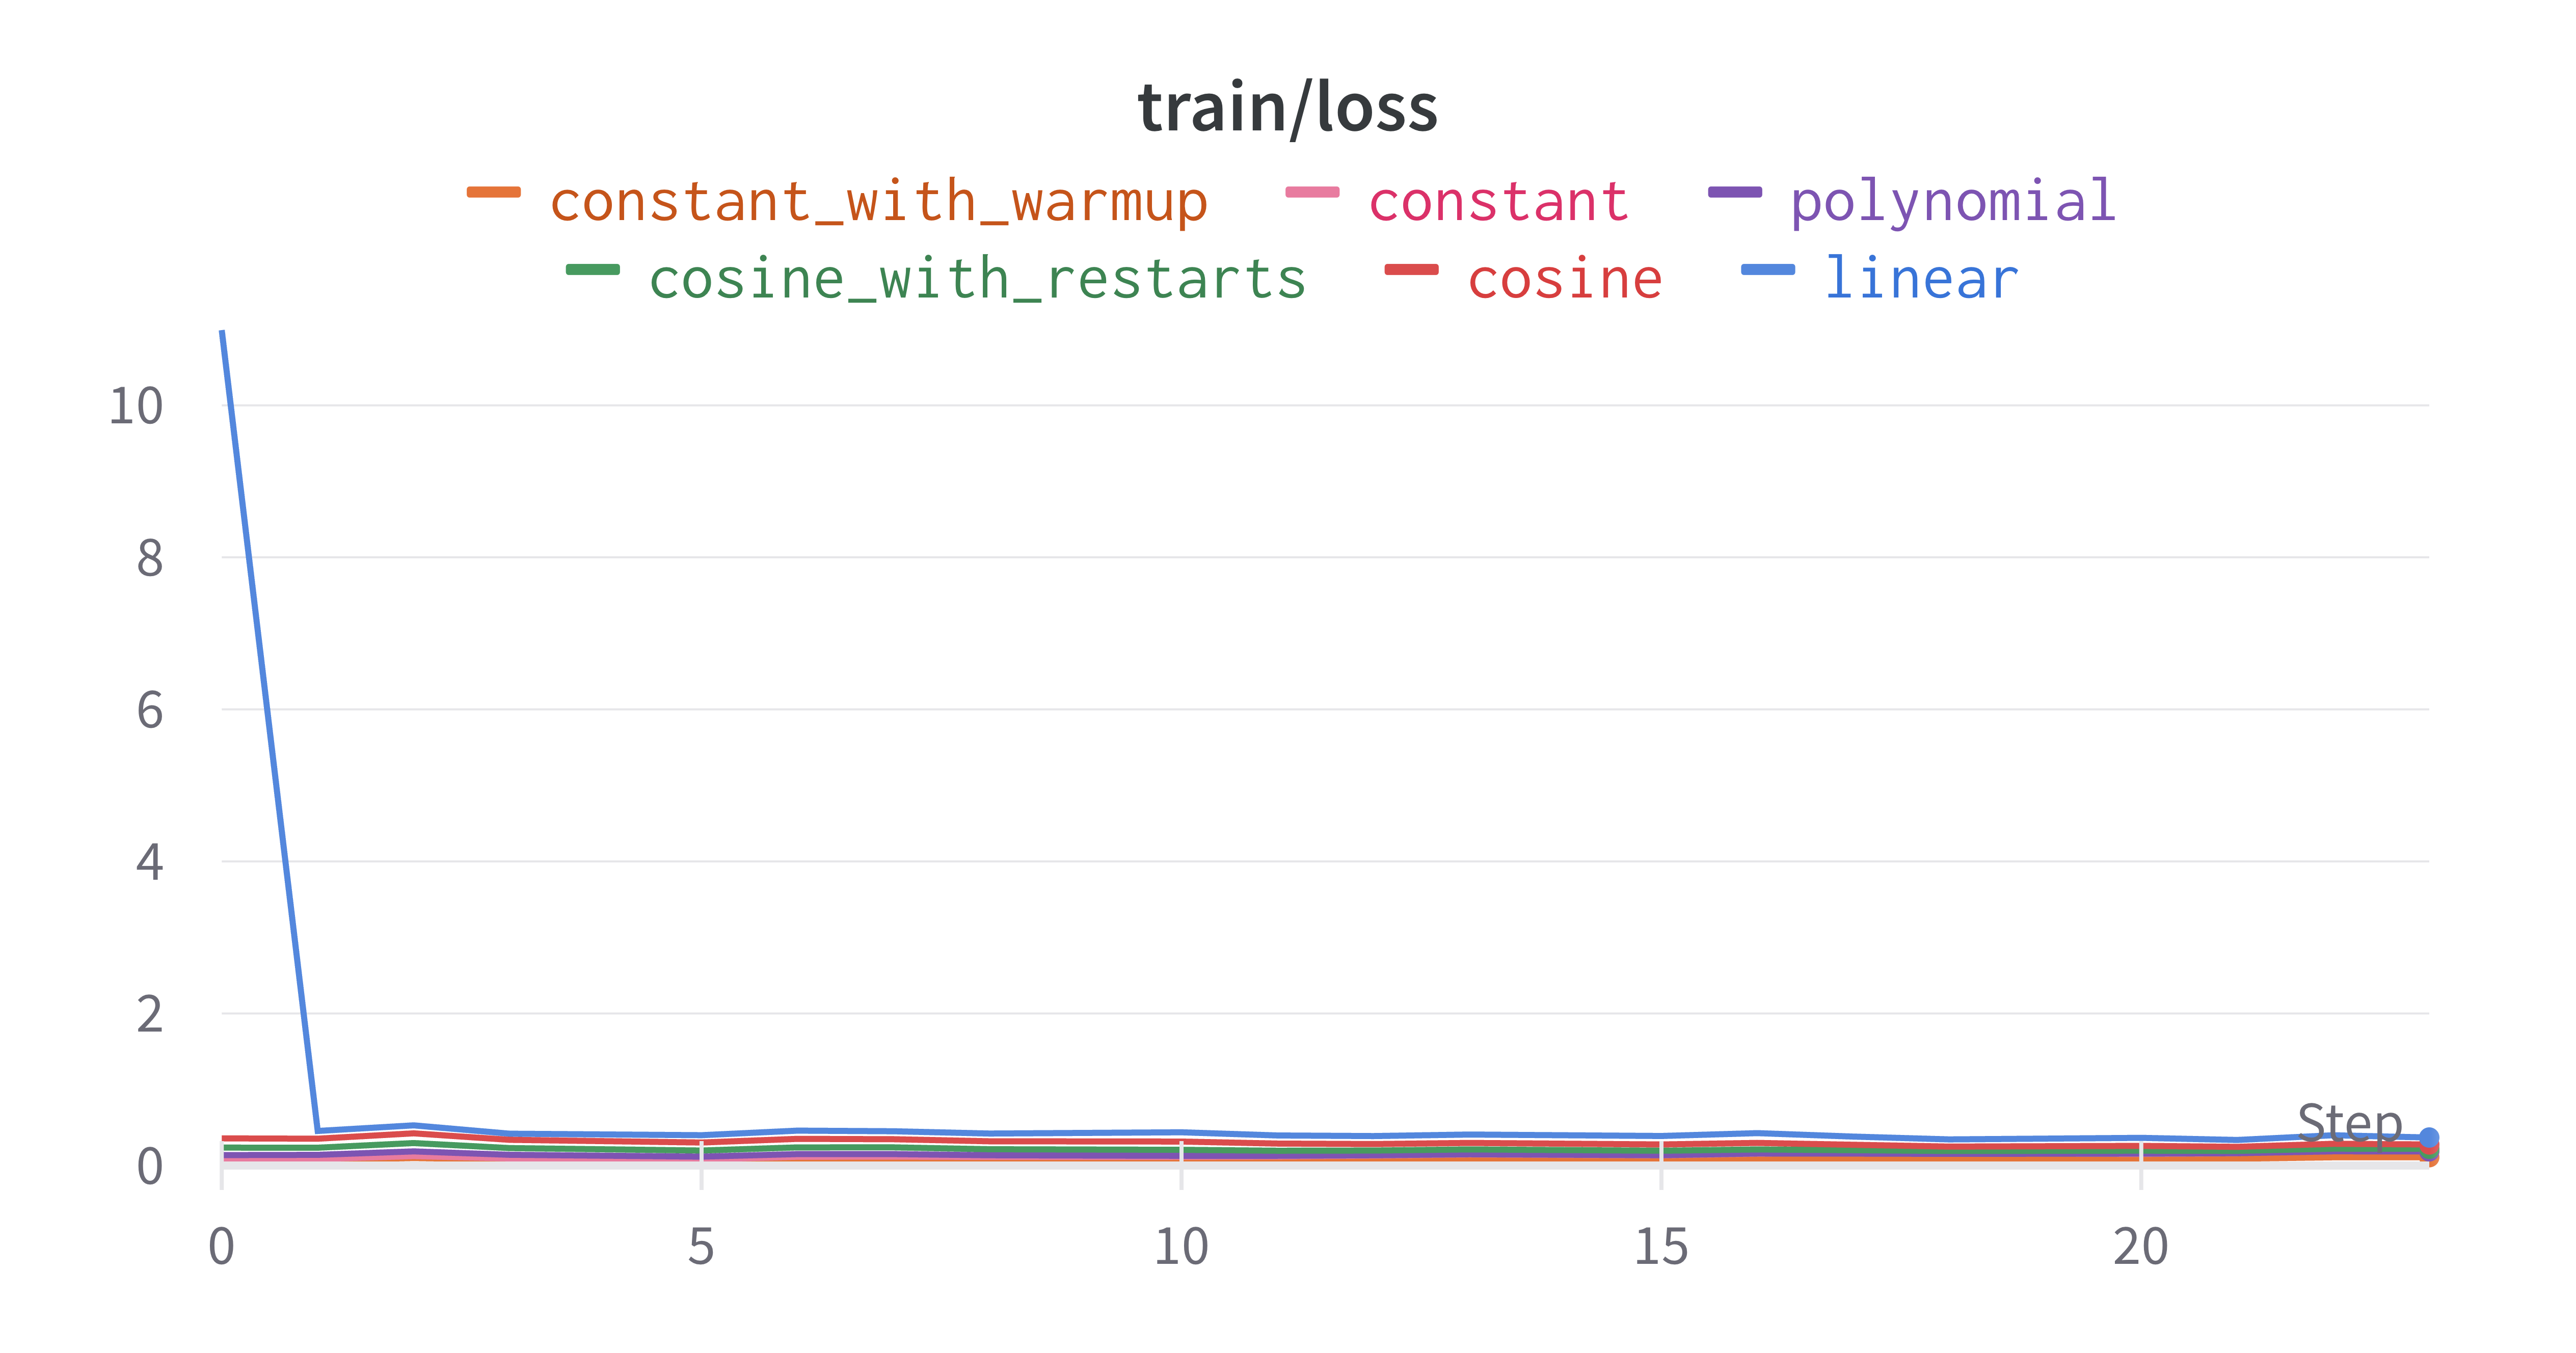
\includegraphics[width=.6\textwidth]{lr-s-train-loss}
  \caption{Значение функции ошибки на тренировочных данных}
  \label{lr-s-train-loss}
\end{figure}

\begin{figure}[!ht]
  \centering
  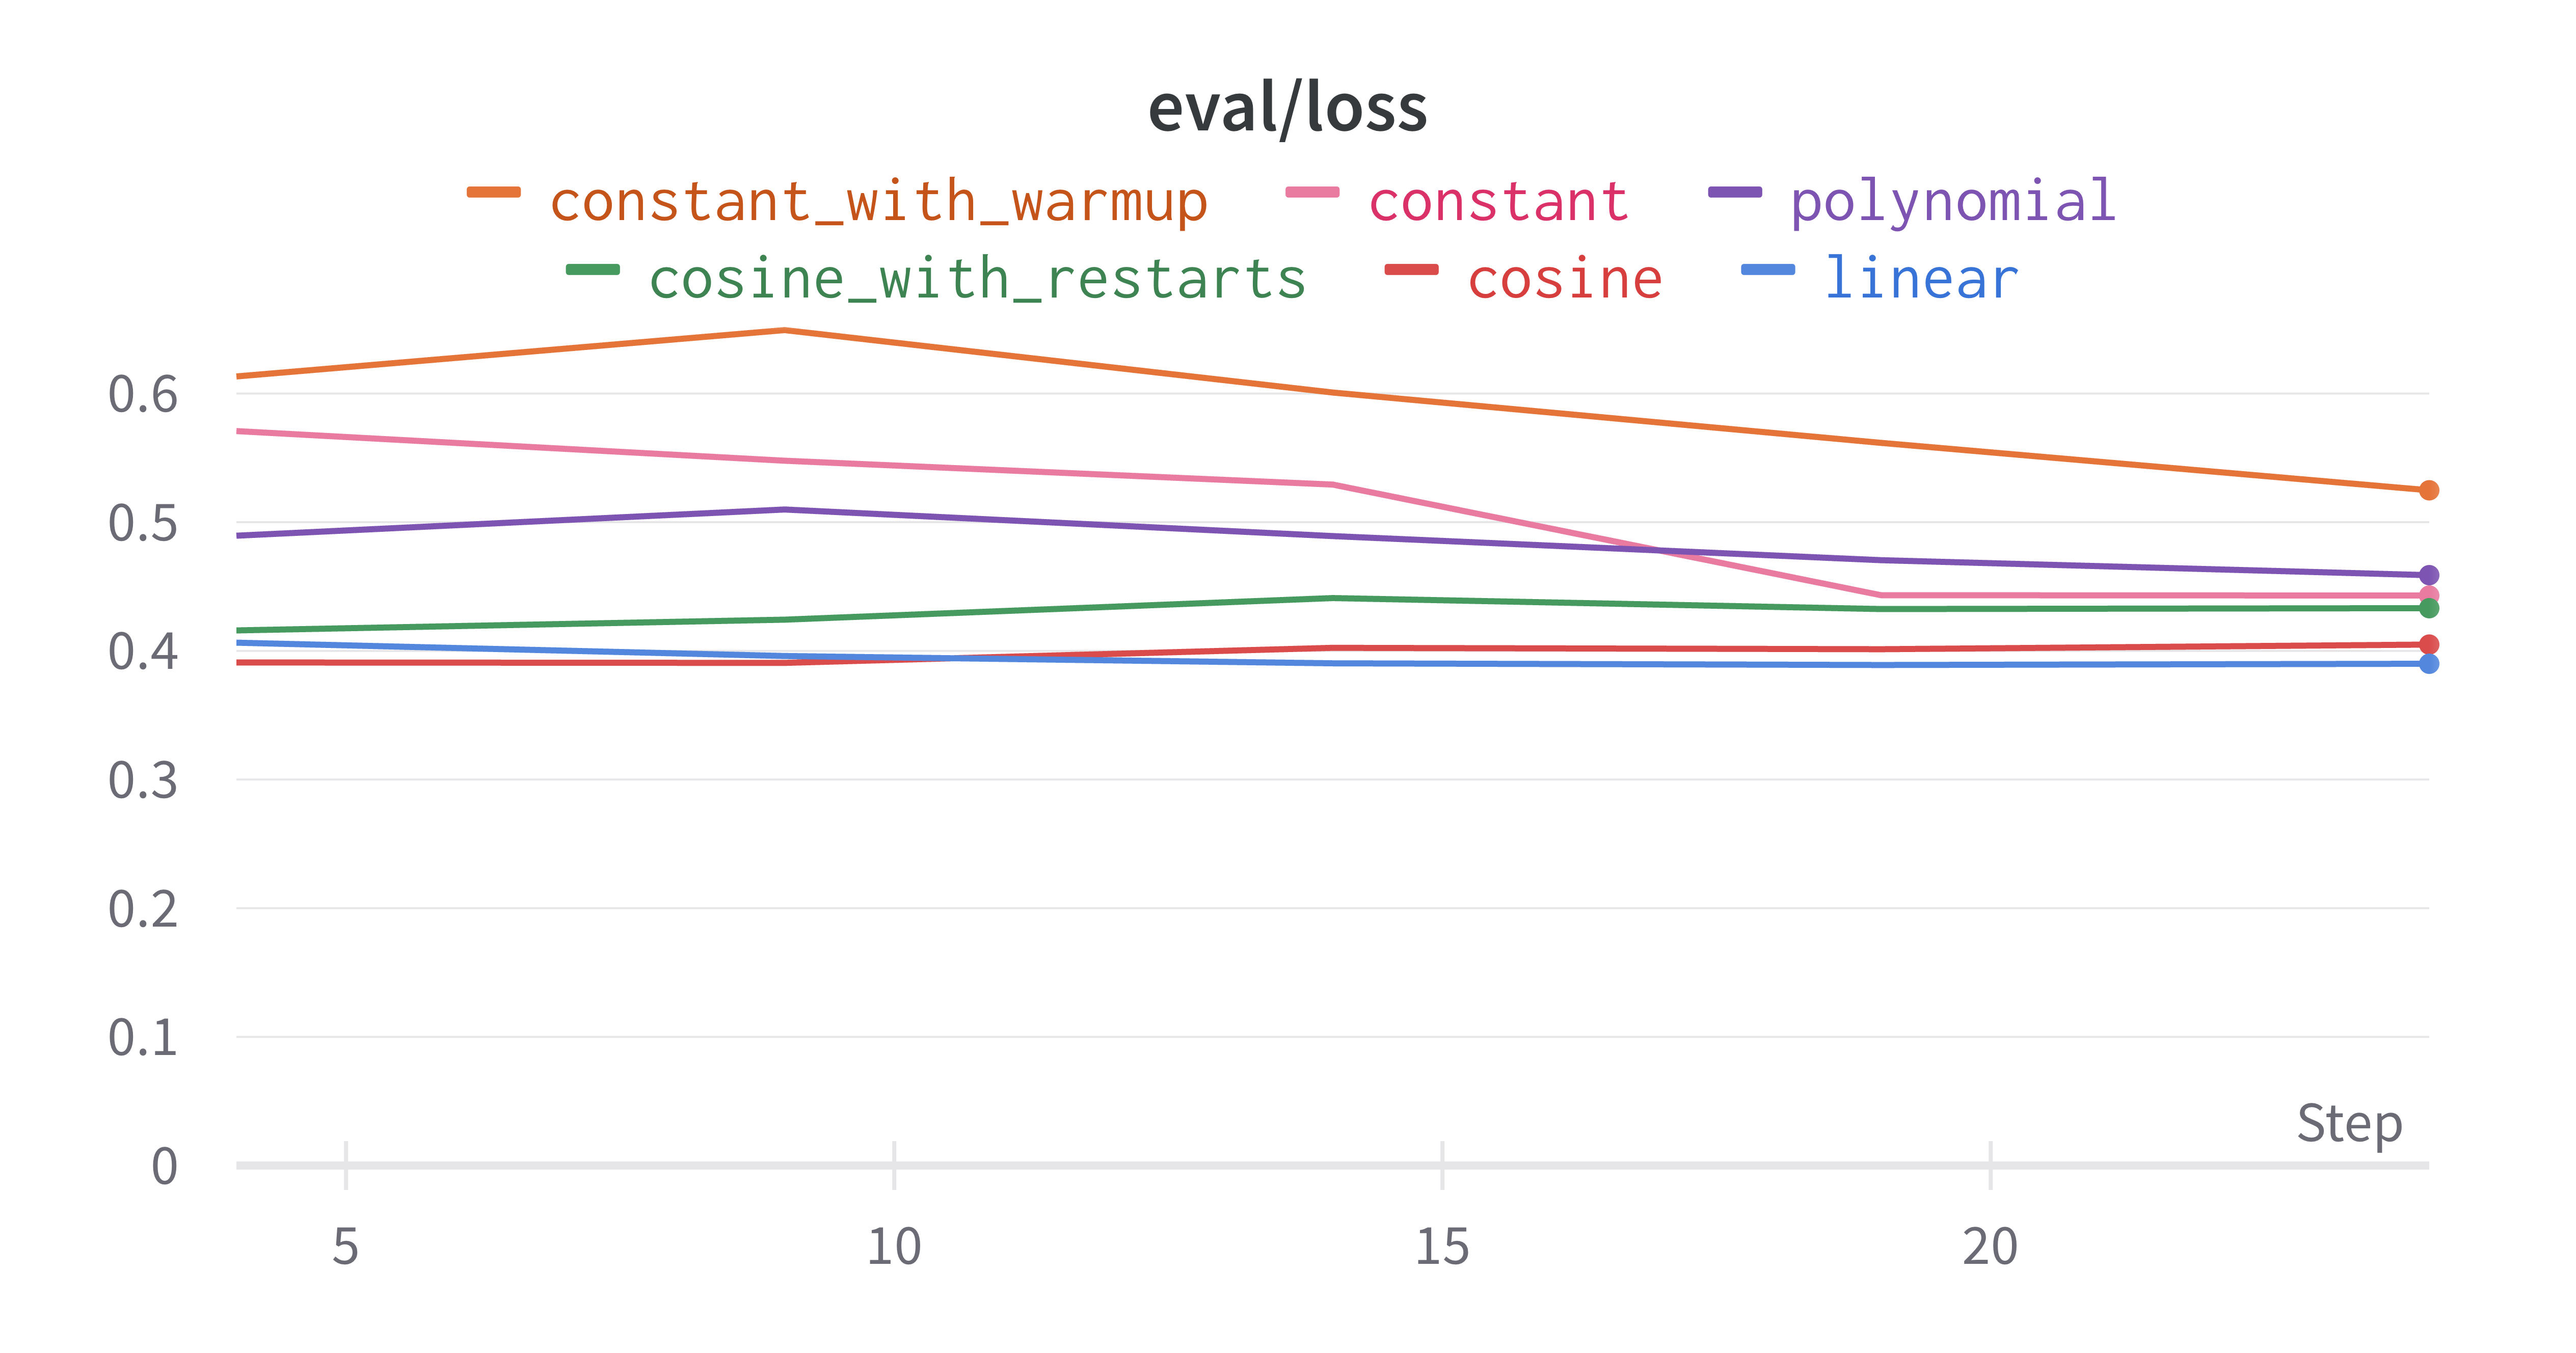
\includegraphics[width=.6\textwidth]{lr-s-eval-loss}
  \caption{Значение функции ошибки на валидационных данных}
  \label{lr-s-eval-loss}
\end{figure}

\begin{figure}[!ht]
  \centering
  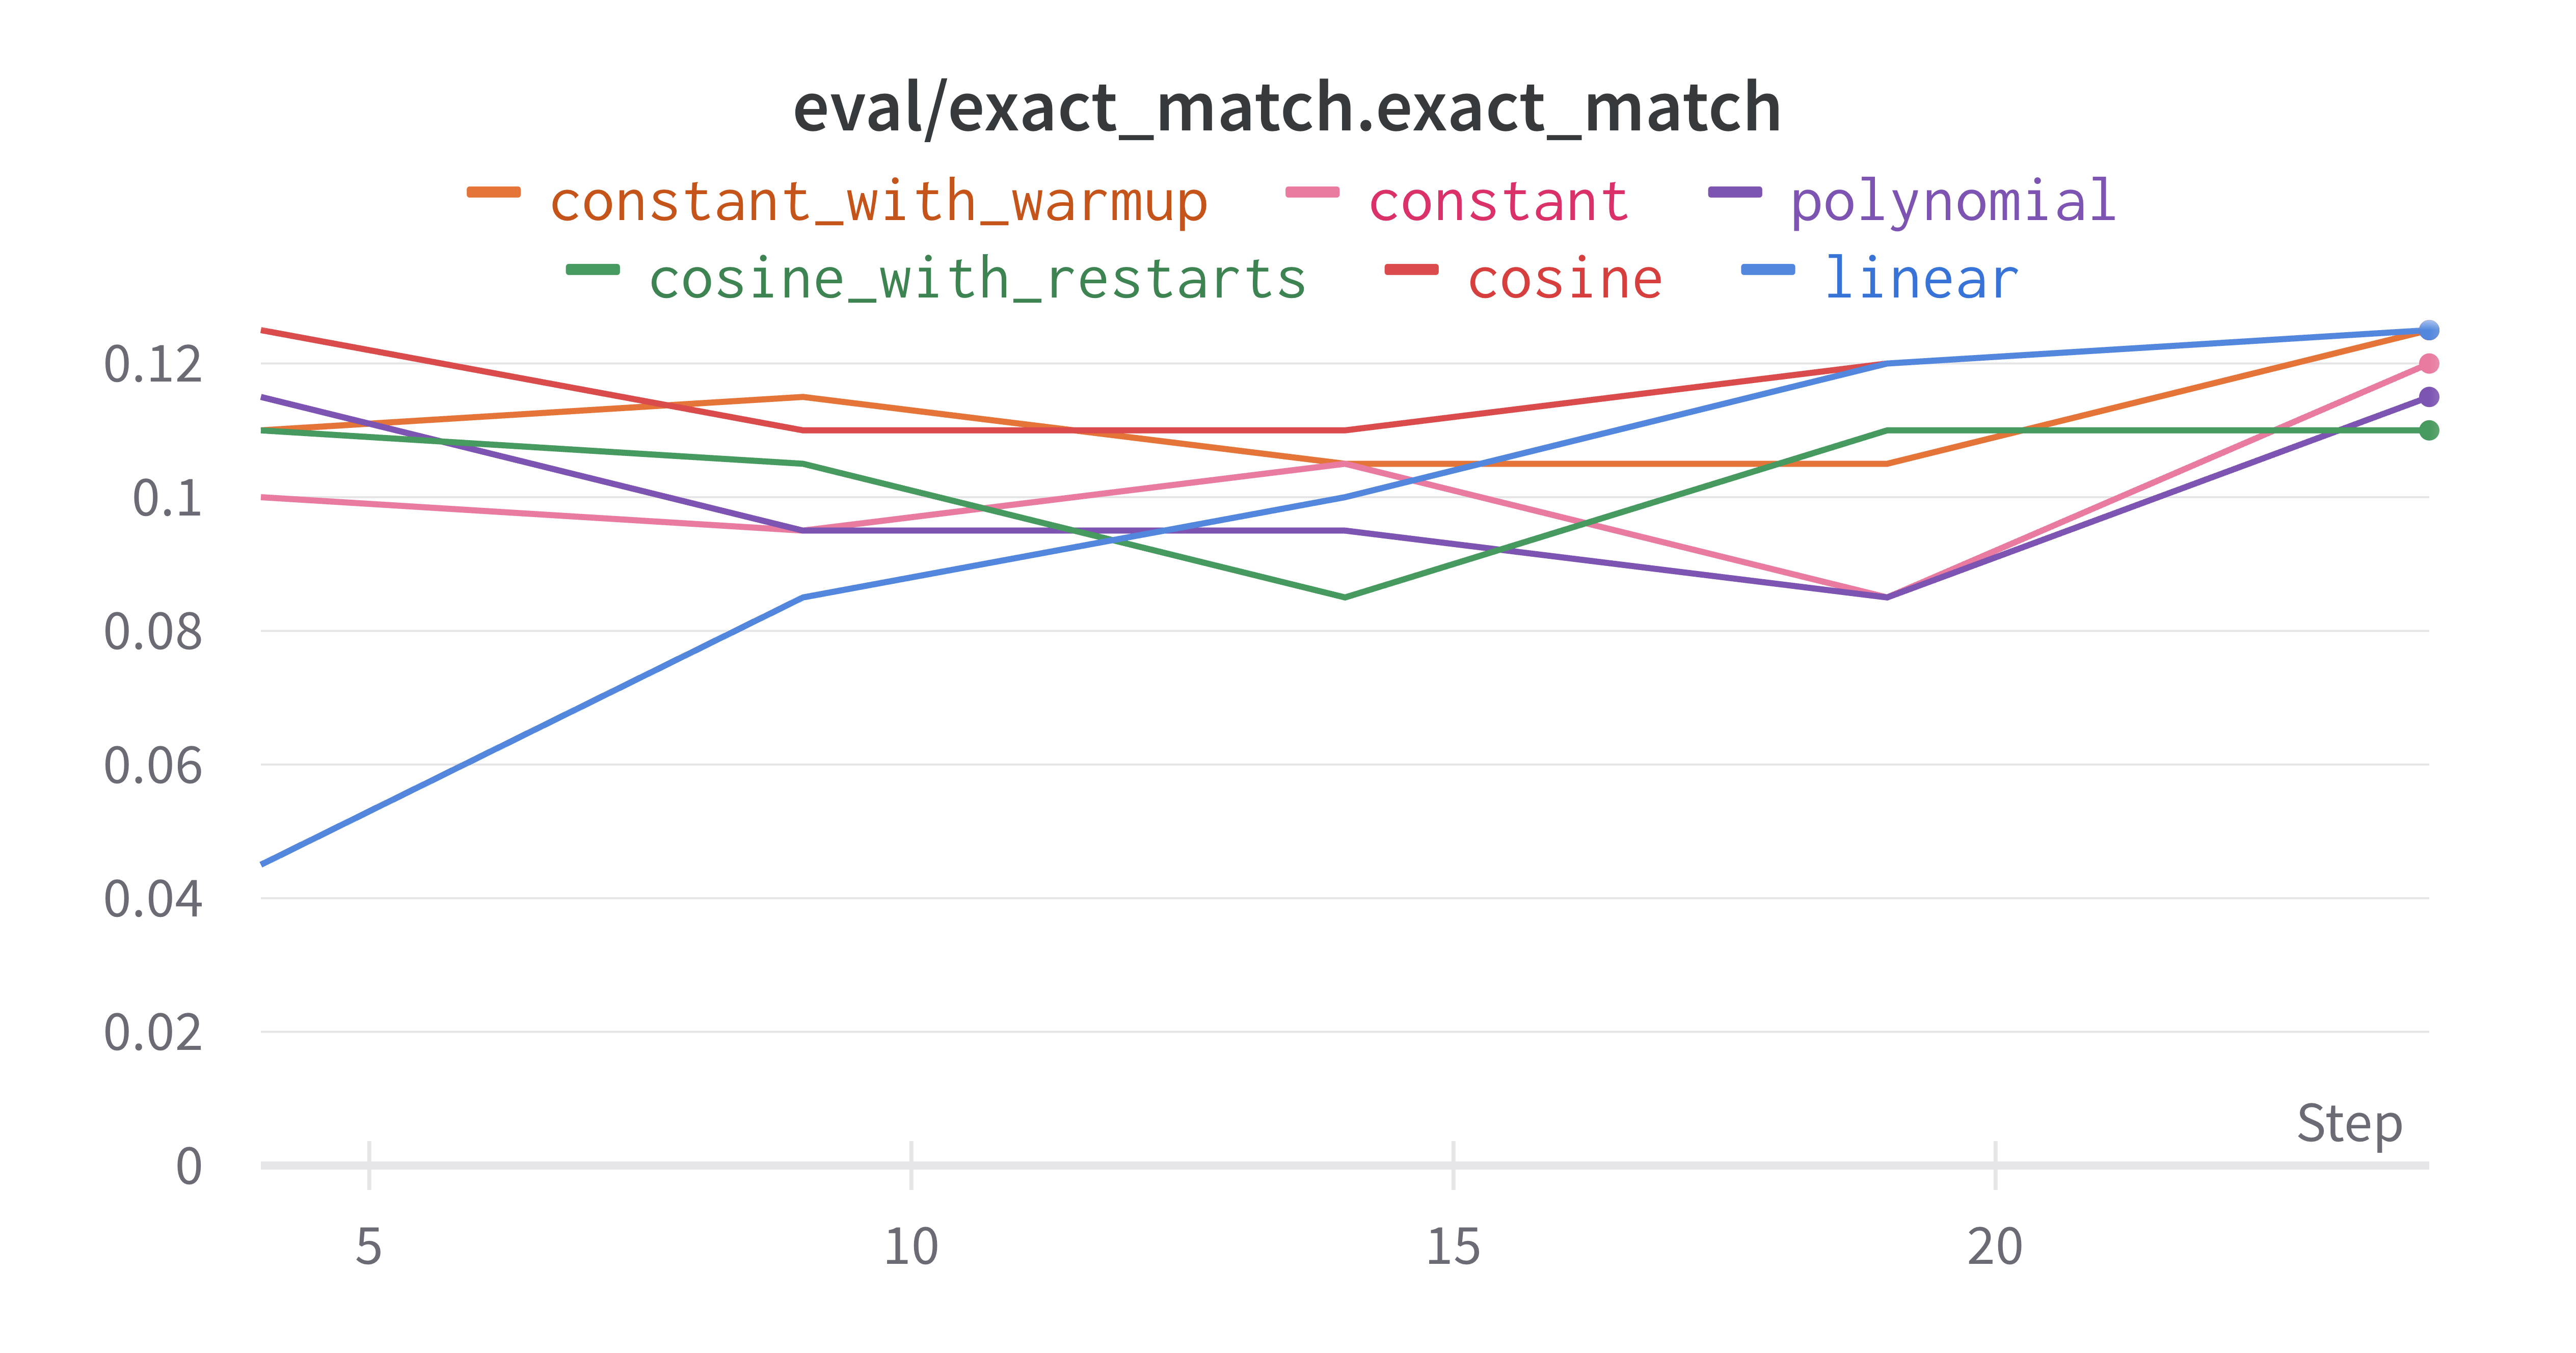
\includegraphics[width=.6\textwidth]{lr-s-em}
  \caption{Значение метрики Exact Match на валидационных данных}
  \label{lr-s-em}
\end{figure}

\begin{figure}[!ht]
  \centering
  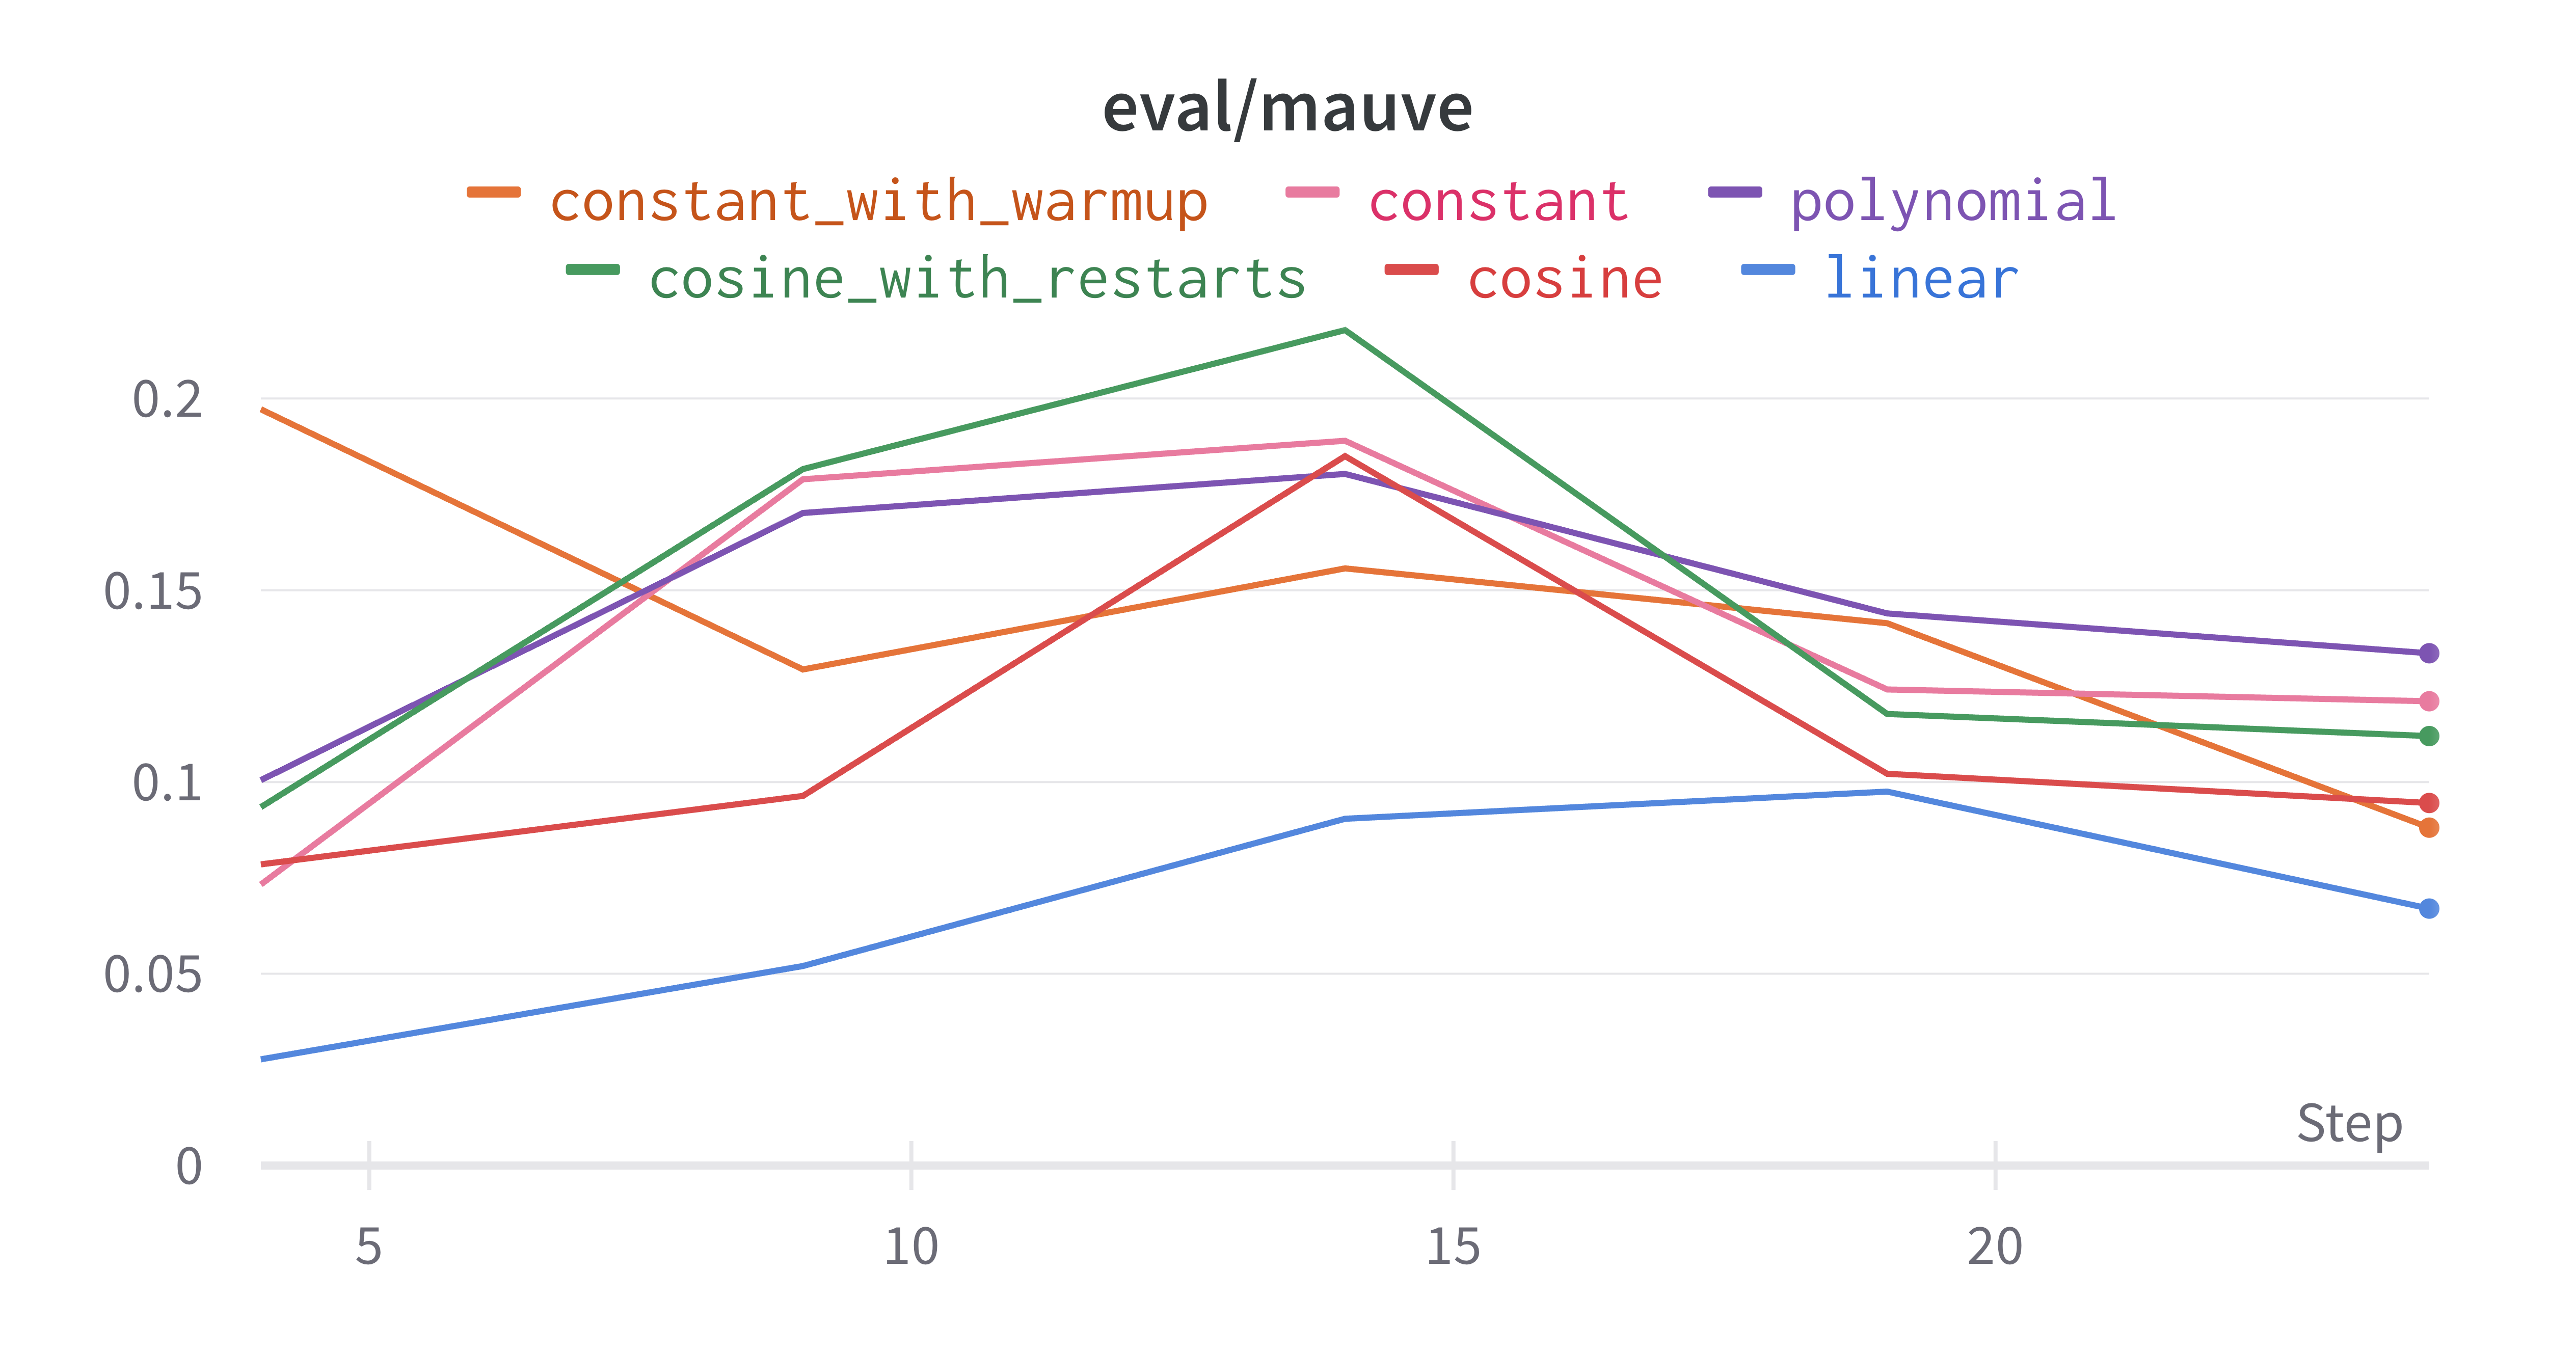
\includegraphics[width=.6\textwidth]{lr-s-mauve}
  \caption{Значение метрики MAUVE на валидационных данных}
  \label{lr-s-mauve}
\end{figure}

\begin{figure}[!ht]
  \centering
  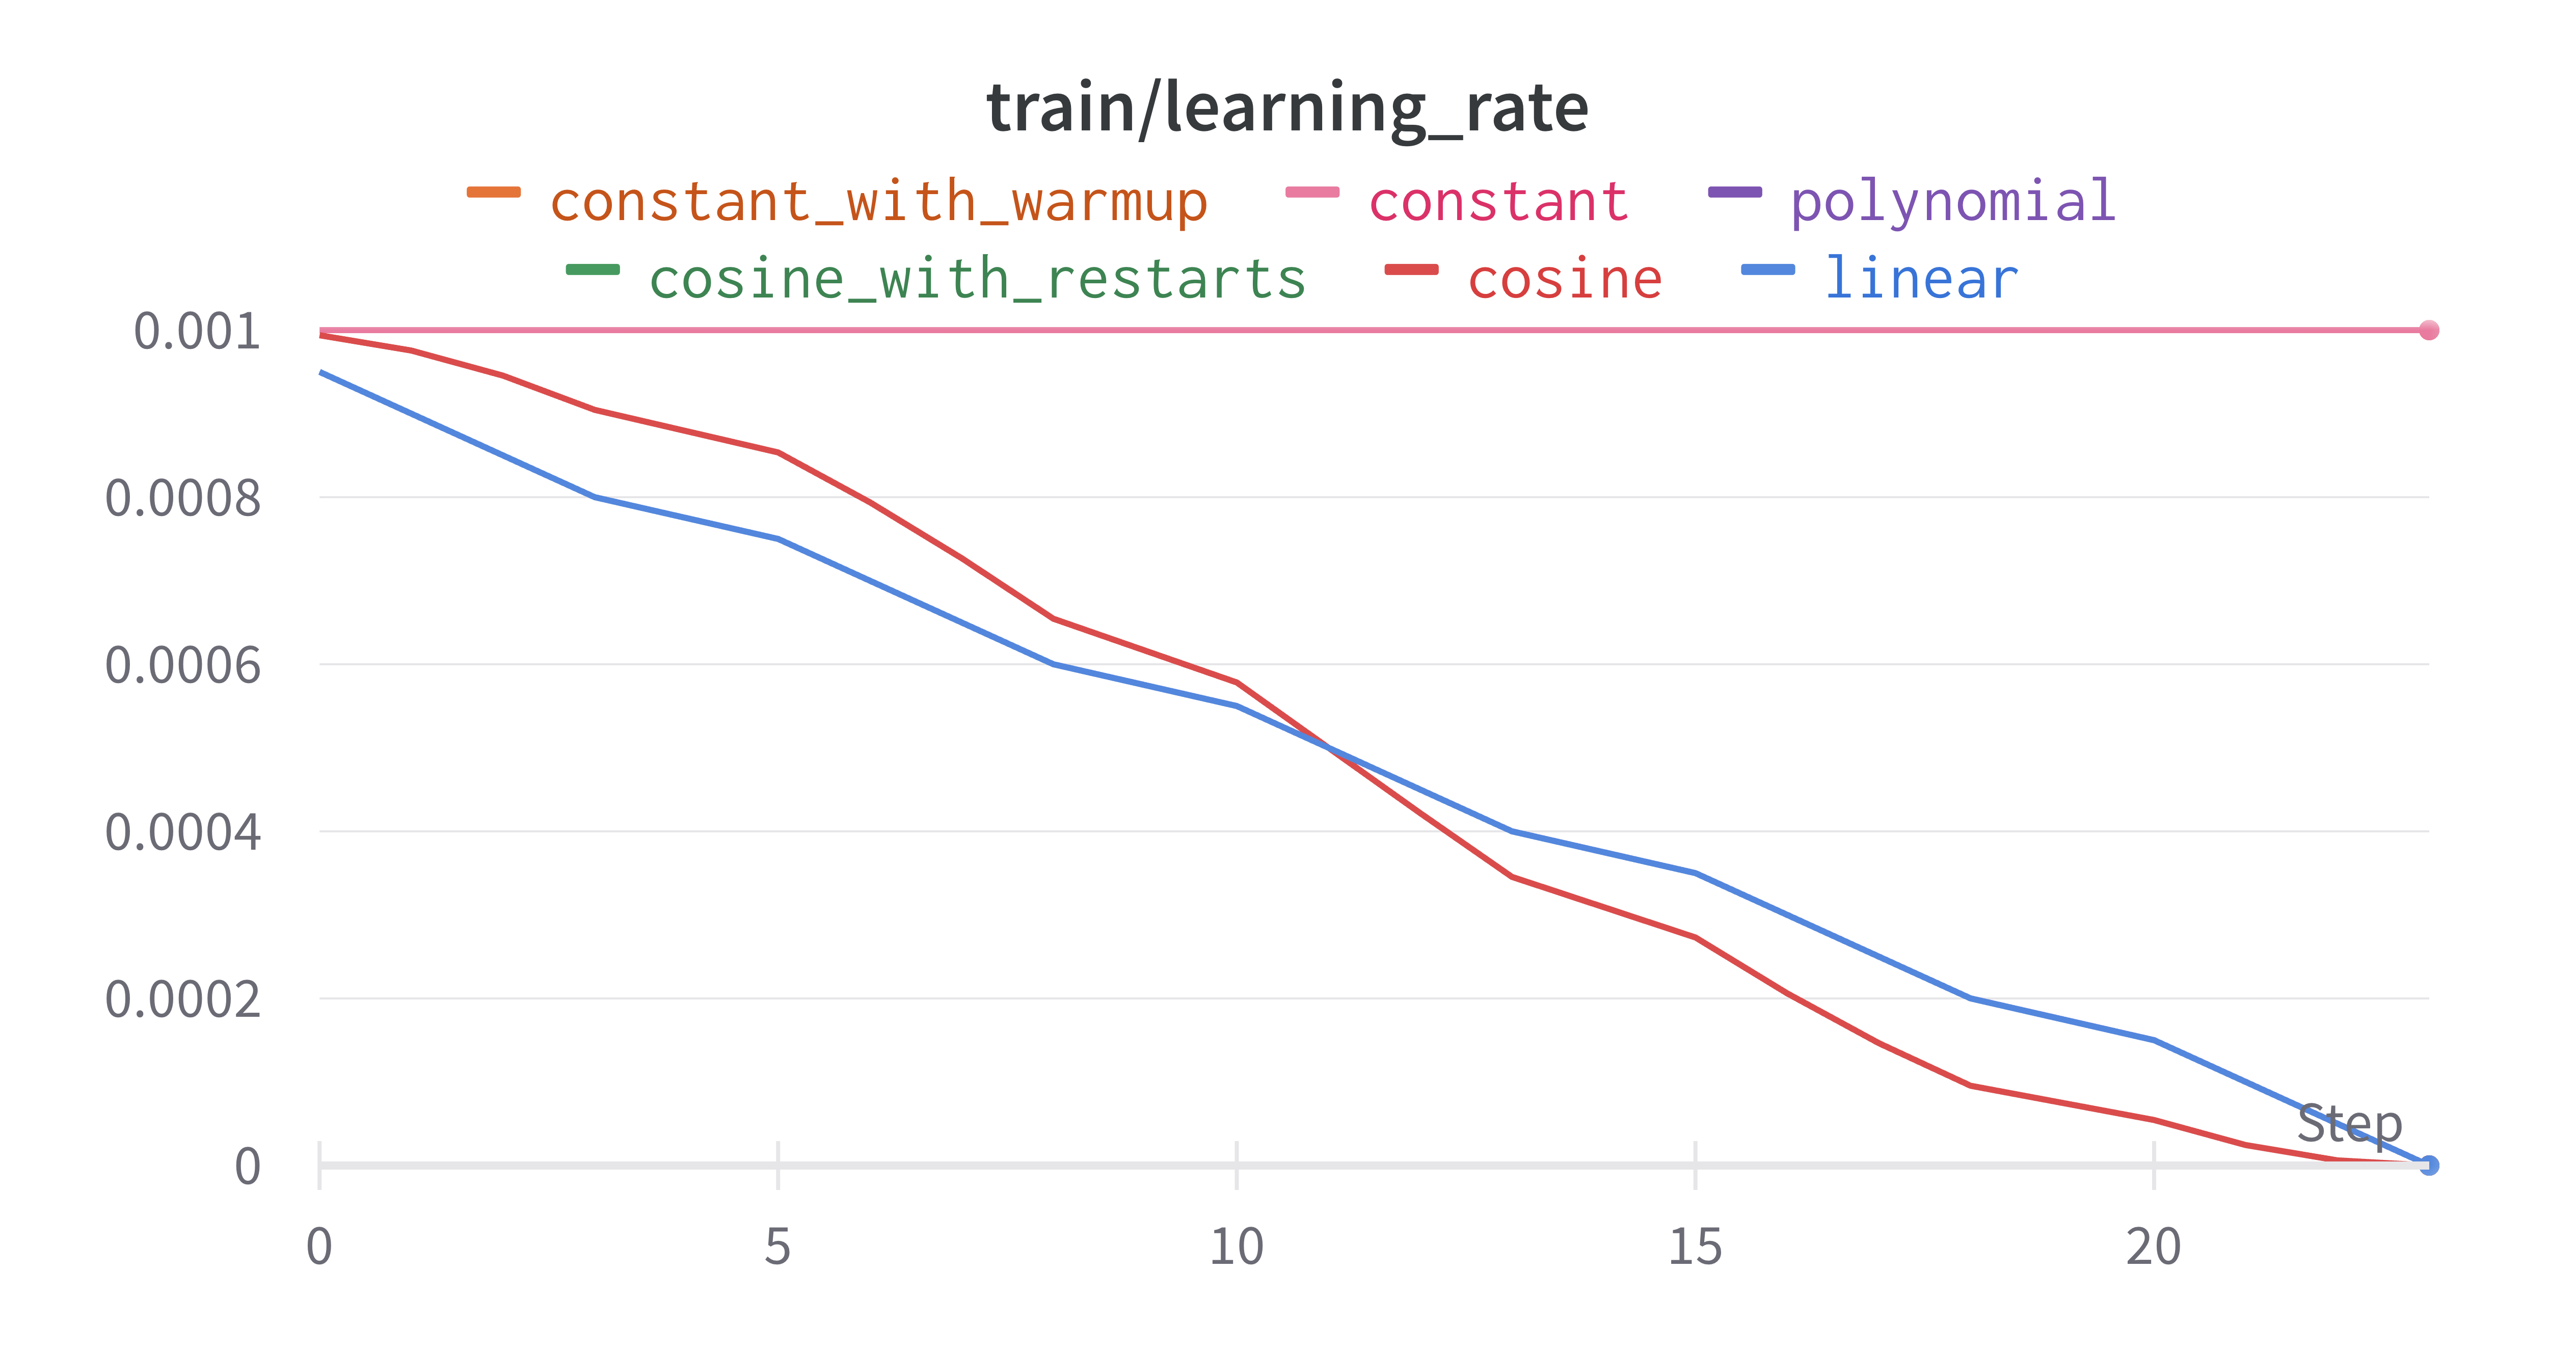
\includegraphics[width=.6\textwidth]{lr-s-lr}
  \caption{График изменения скорости обучения}
  \label{lr-s-lr}
\end{figure}

В следующих экспериментах при зафиксированном константном планировщике скорости обучения искалась наиболее эффективная скорость обучения. Стоит отметить, что при скорости обучения равной $1 \times 10^{-4}$ процесс обучения не завершился успешно. Из рисунков \ref{lr-train-loss}, \ref{lr-eval-loss}, \ref{lr-em}, \ref{lr-mauve} видно, что значения, близкие к $4 \times 10^{-4}$ и к $9 \times 10^{-4}$ показывают лучшие значения функций ошибок на всех выборках и лучшие значения метрик. Значение скорости обучения $9 \times 10^{-4}$ показывает результаты чуть лучше, чем $4 \times 10^{-4}$, быстрее достигая лучших значений. В целом, почти все значения скорости обучения показывают схожие результаты, но выбор оптимальных параметров для обучения на большей выборке может сказаться на качестве модели.

% LR
\begin{figure}[!ht]
  \centering
  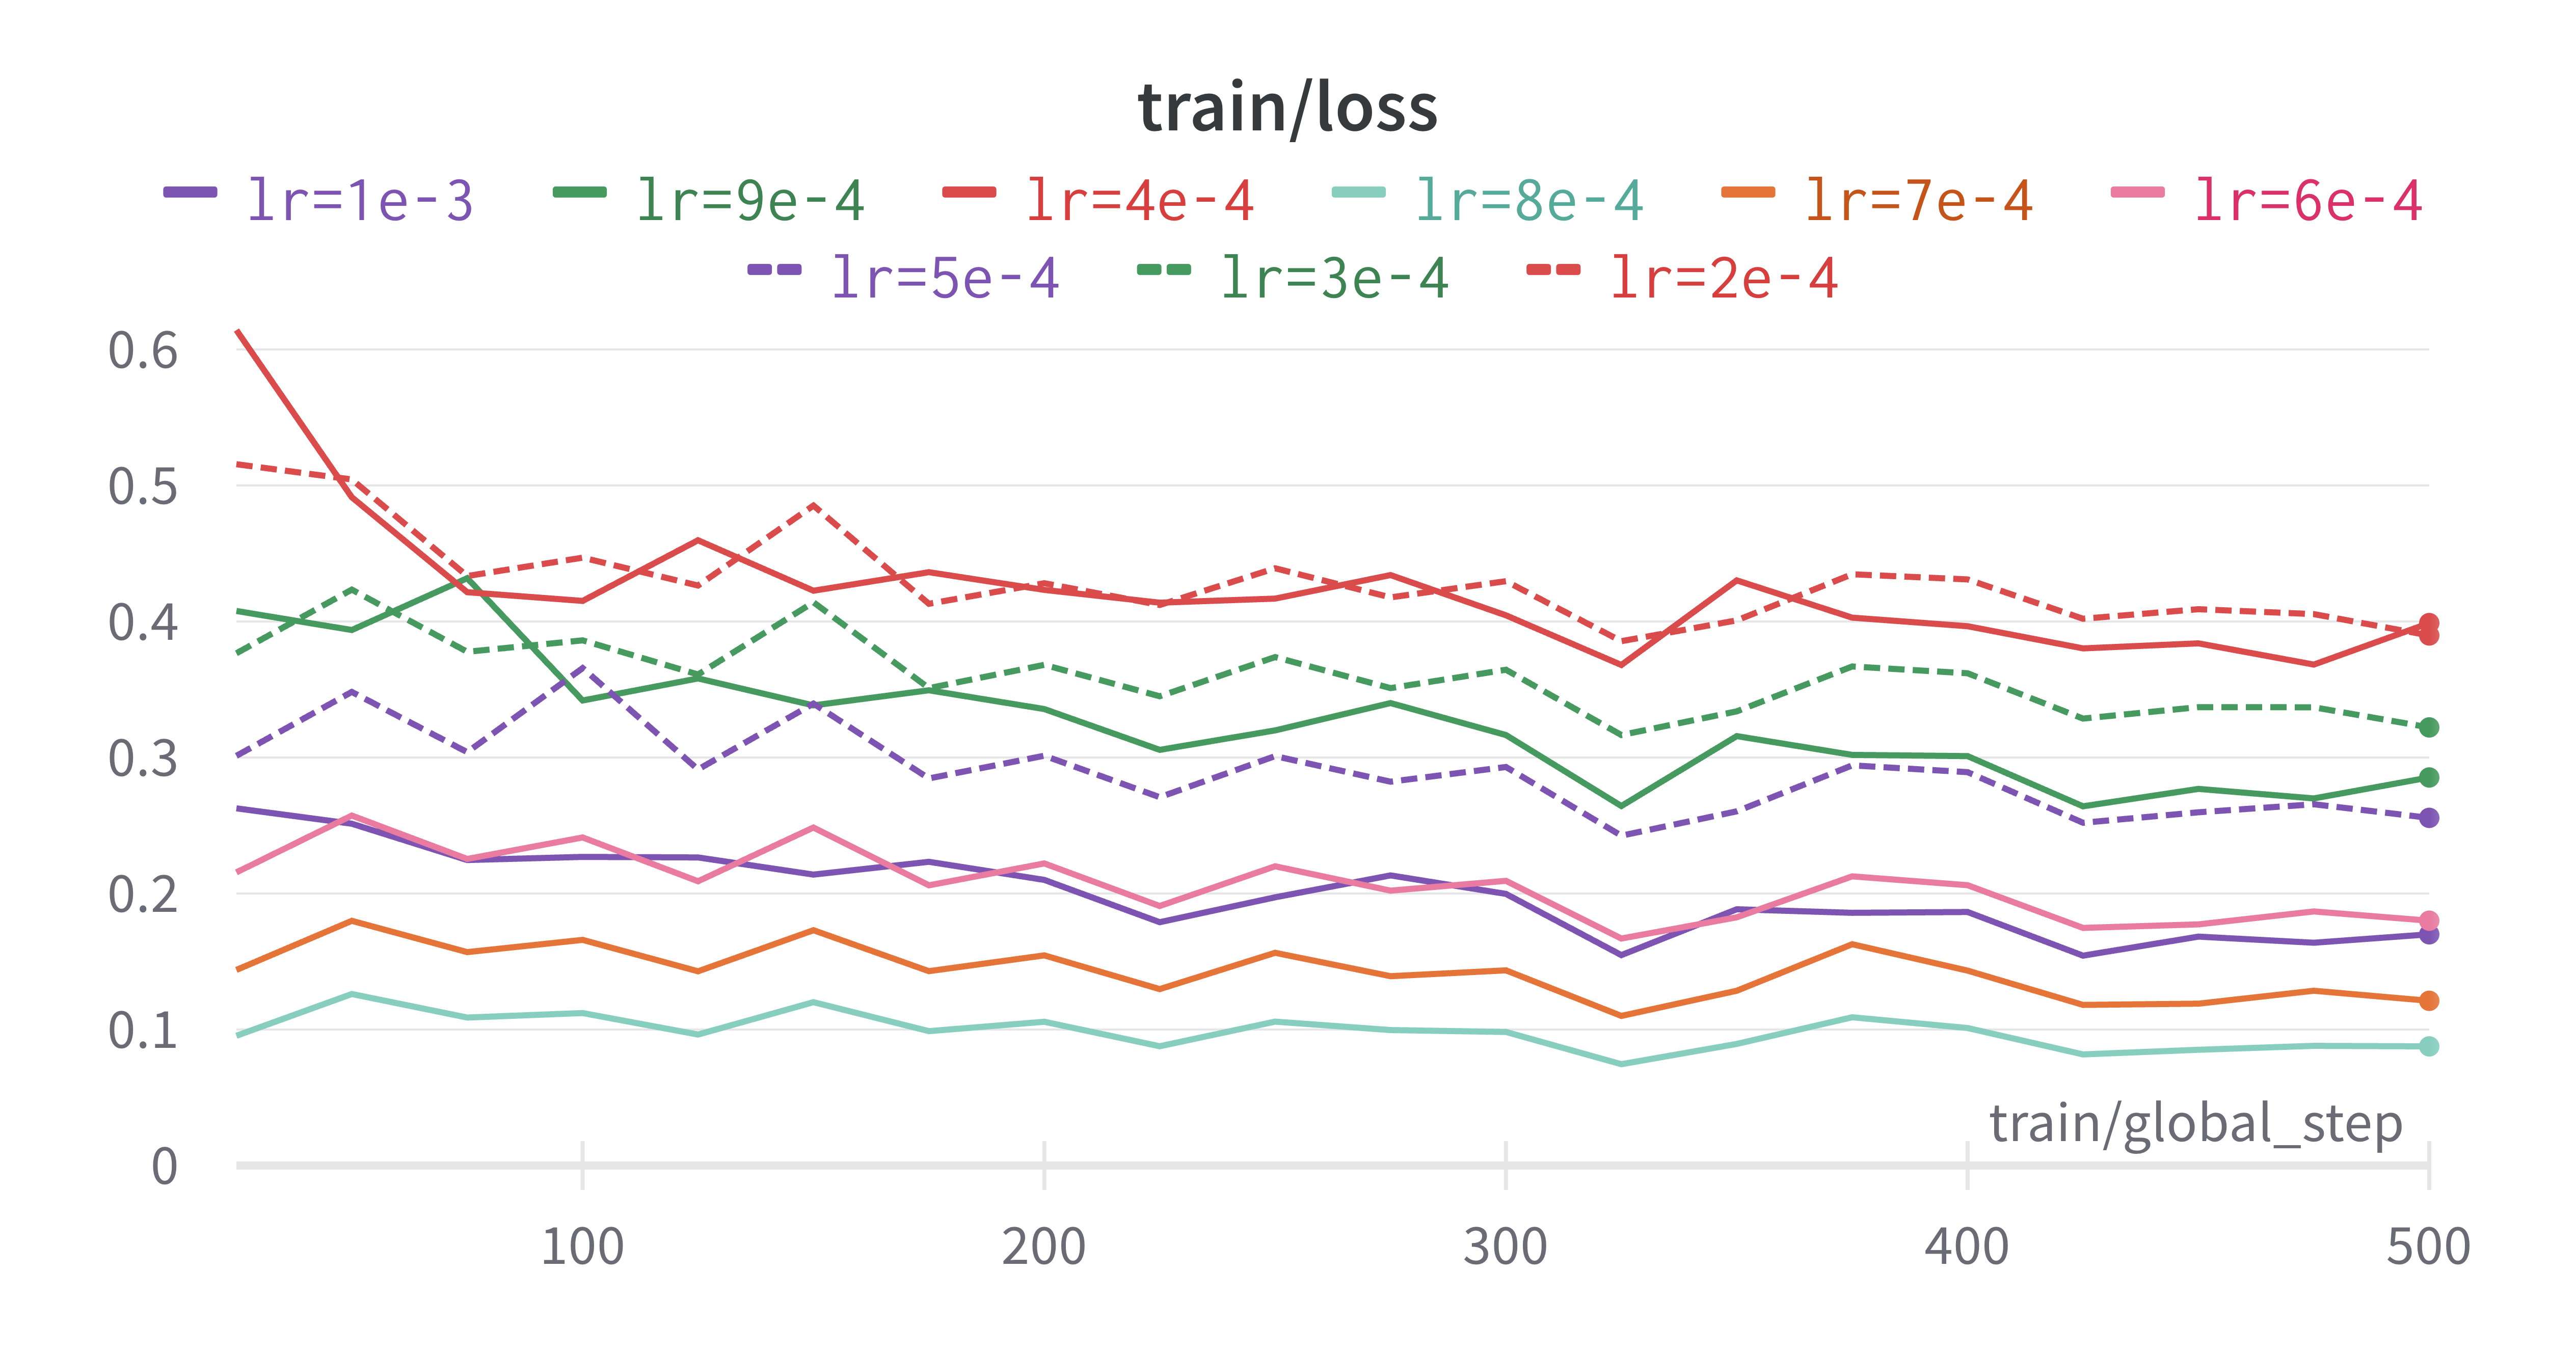
\includegraphics[width=.6\textwidth]{lr-train-loss}
  \caption{Значение функции ошибки на тренировочных данных}
  \label{lr-train-loss}
\end{figure}

\begin{figure}[!ht]
  \centering
  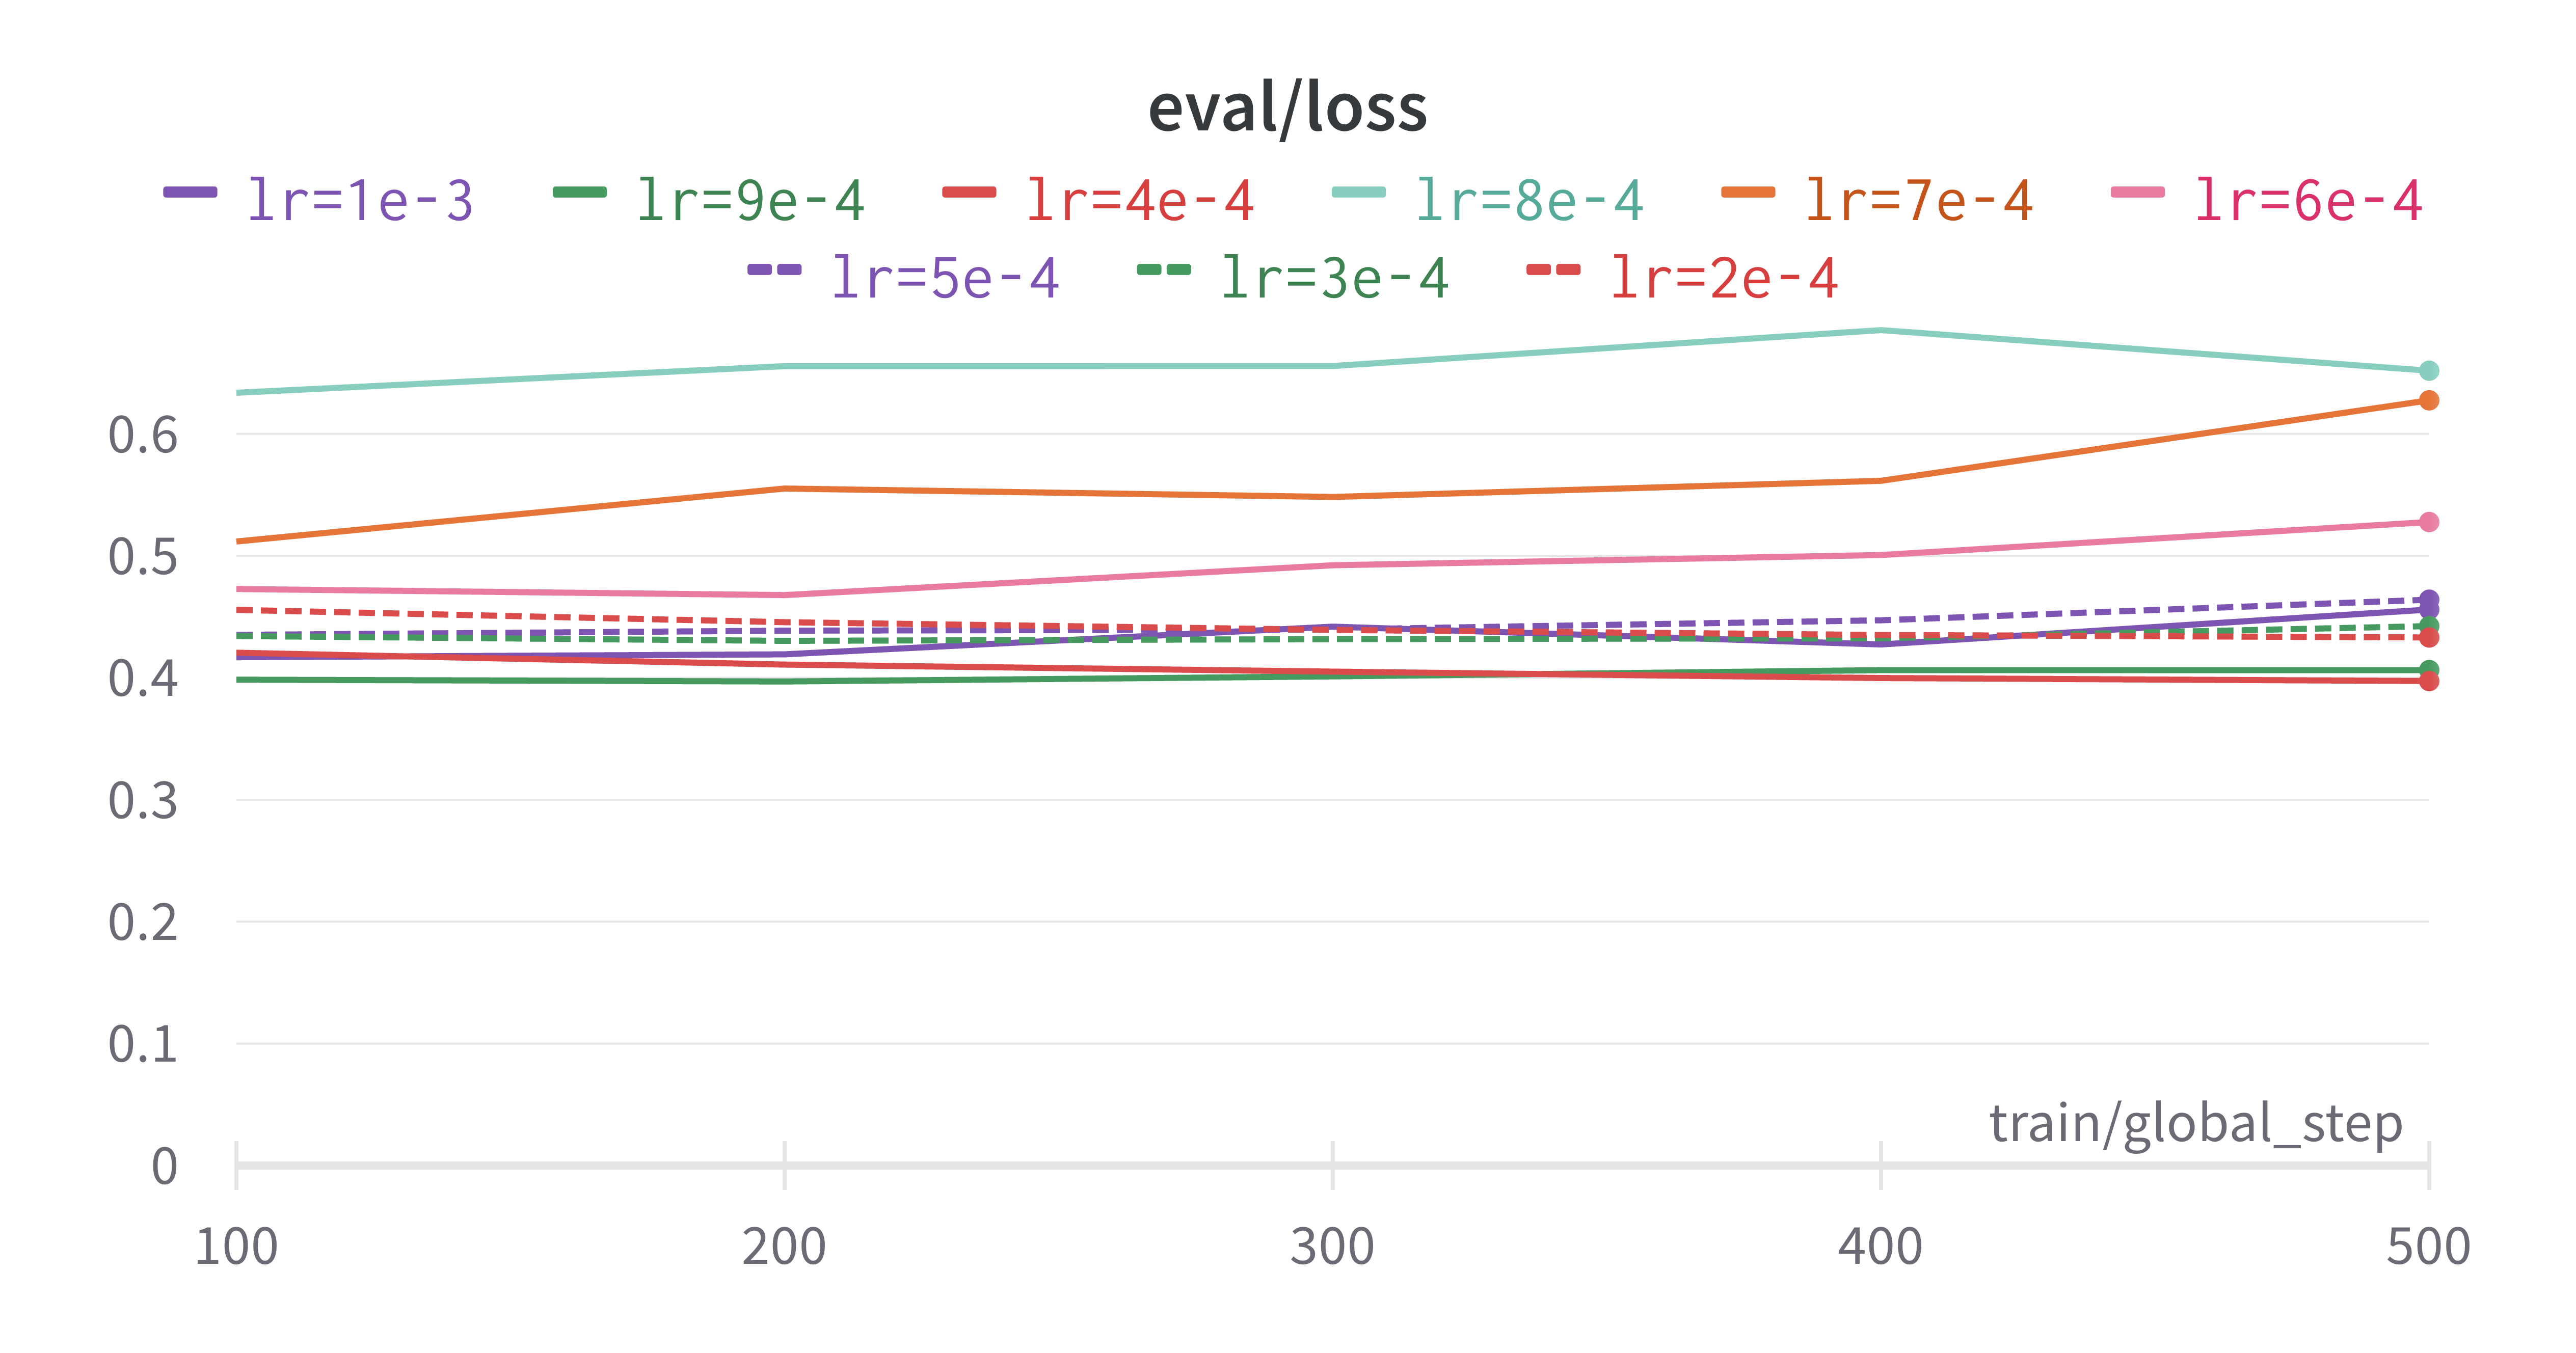
\includegraphics[width=.6\textwidth]{lr-eval-loss}
  \caption{Значение функции ошибки на валидационных данных}
  \label{lr-eval-loss}
\end{figure}

\begin{figure}[!ht]
  \centering
  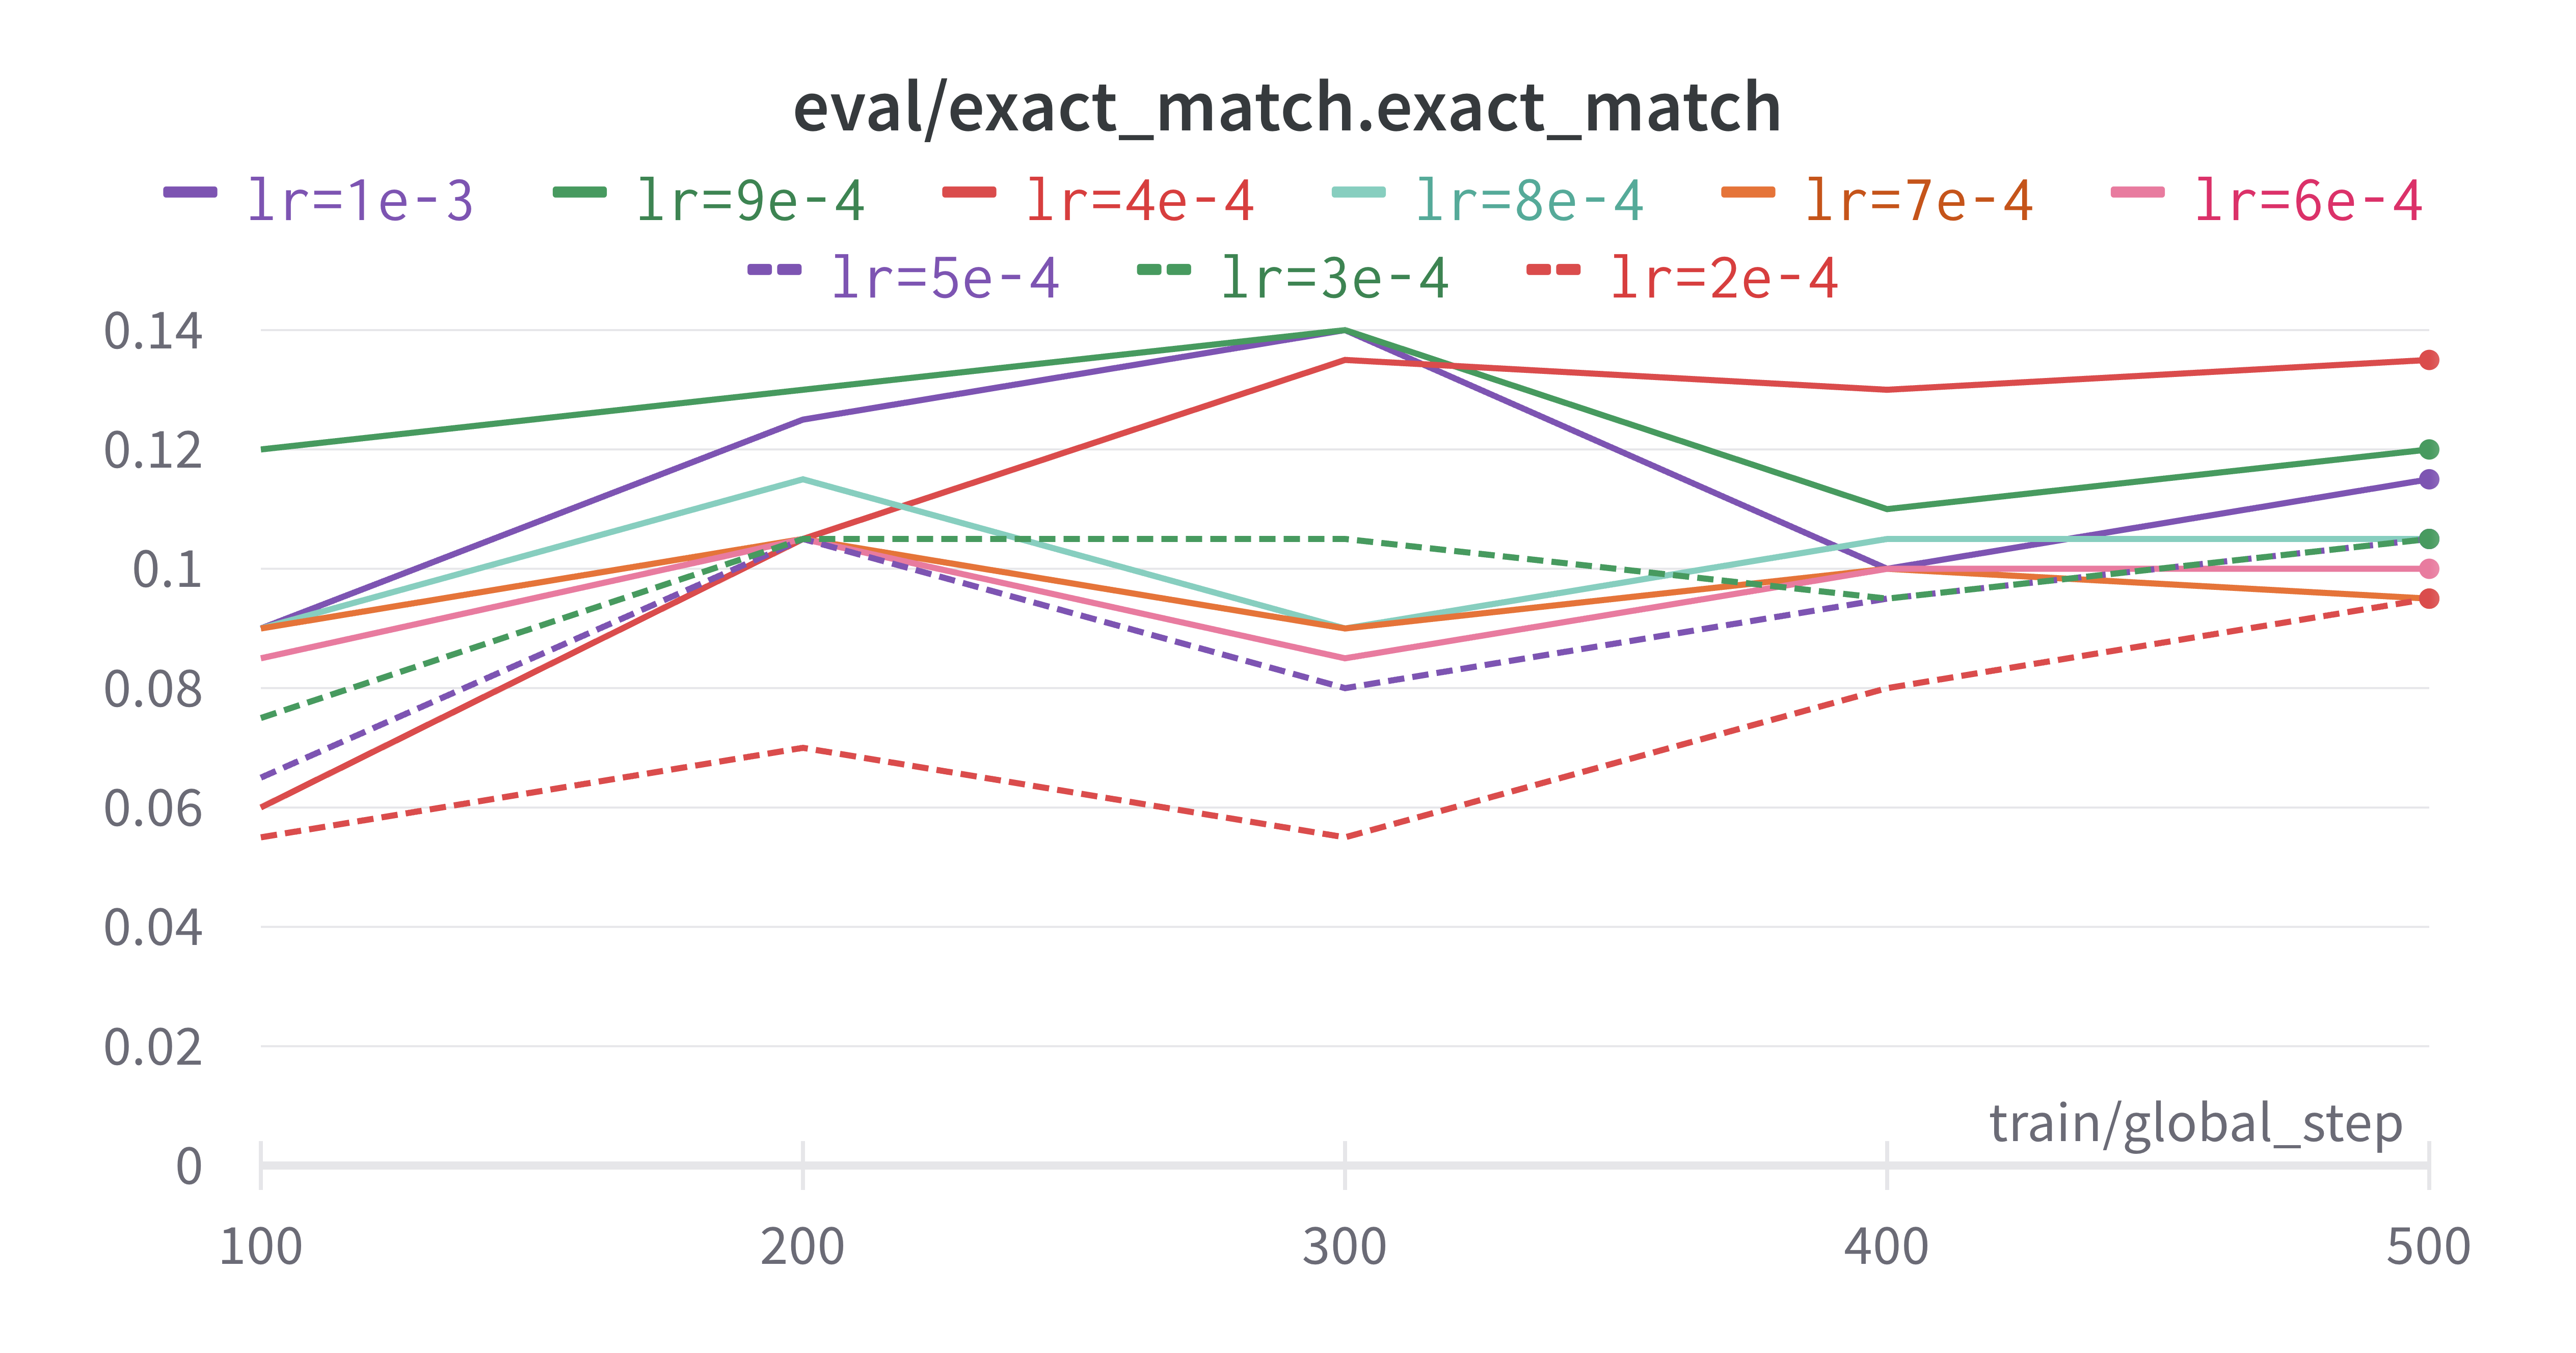
\includegraphics[width=.6\textwidth]{lr-em}
  \caption{Значение метрики Exact Match на валидационных данных}
  \label{lr-em}
\end{figure}

\begin{figure}[!ht]
  \centering
  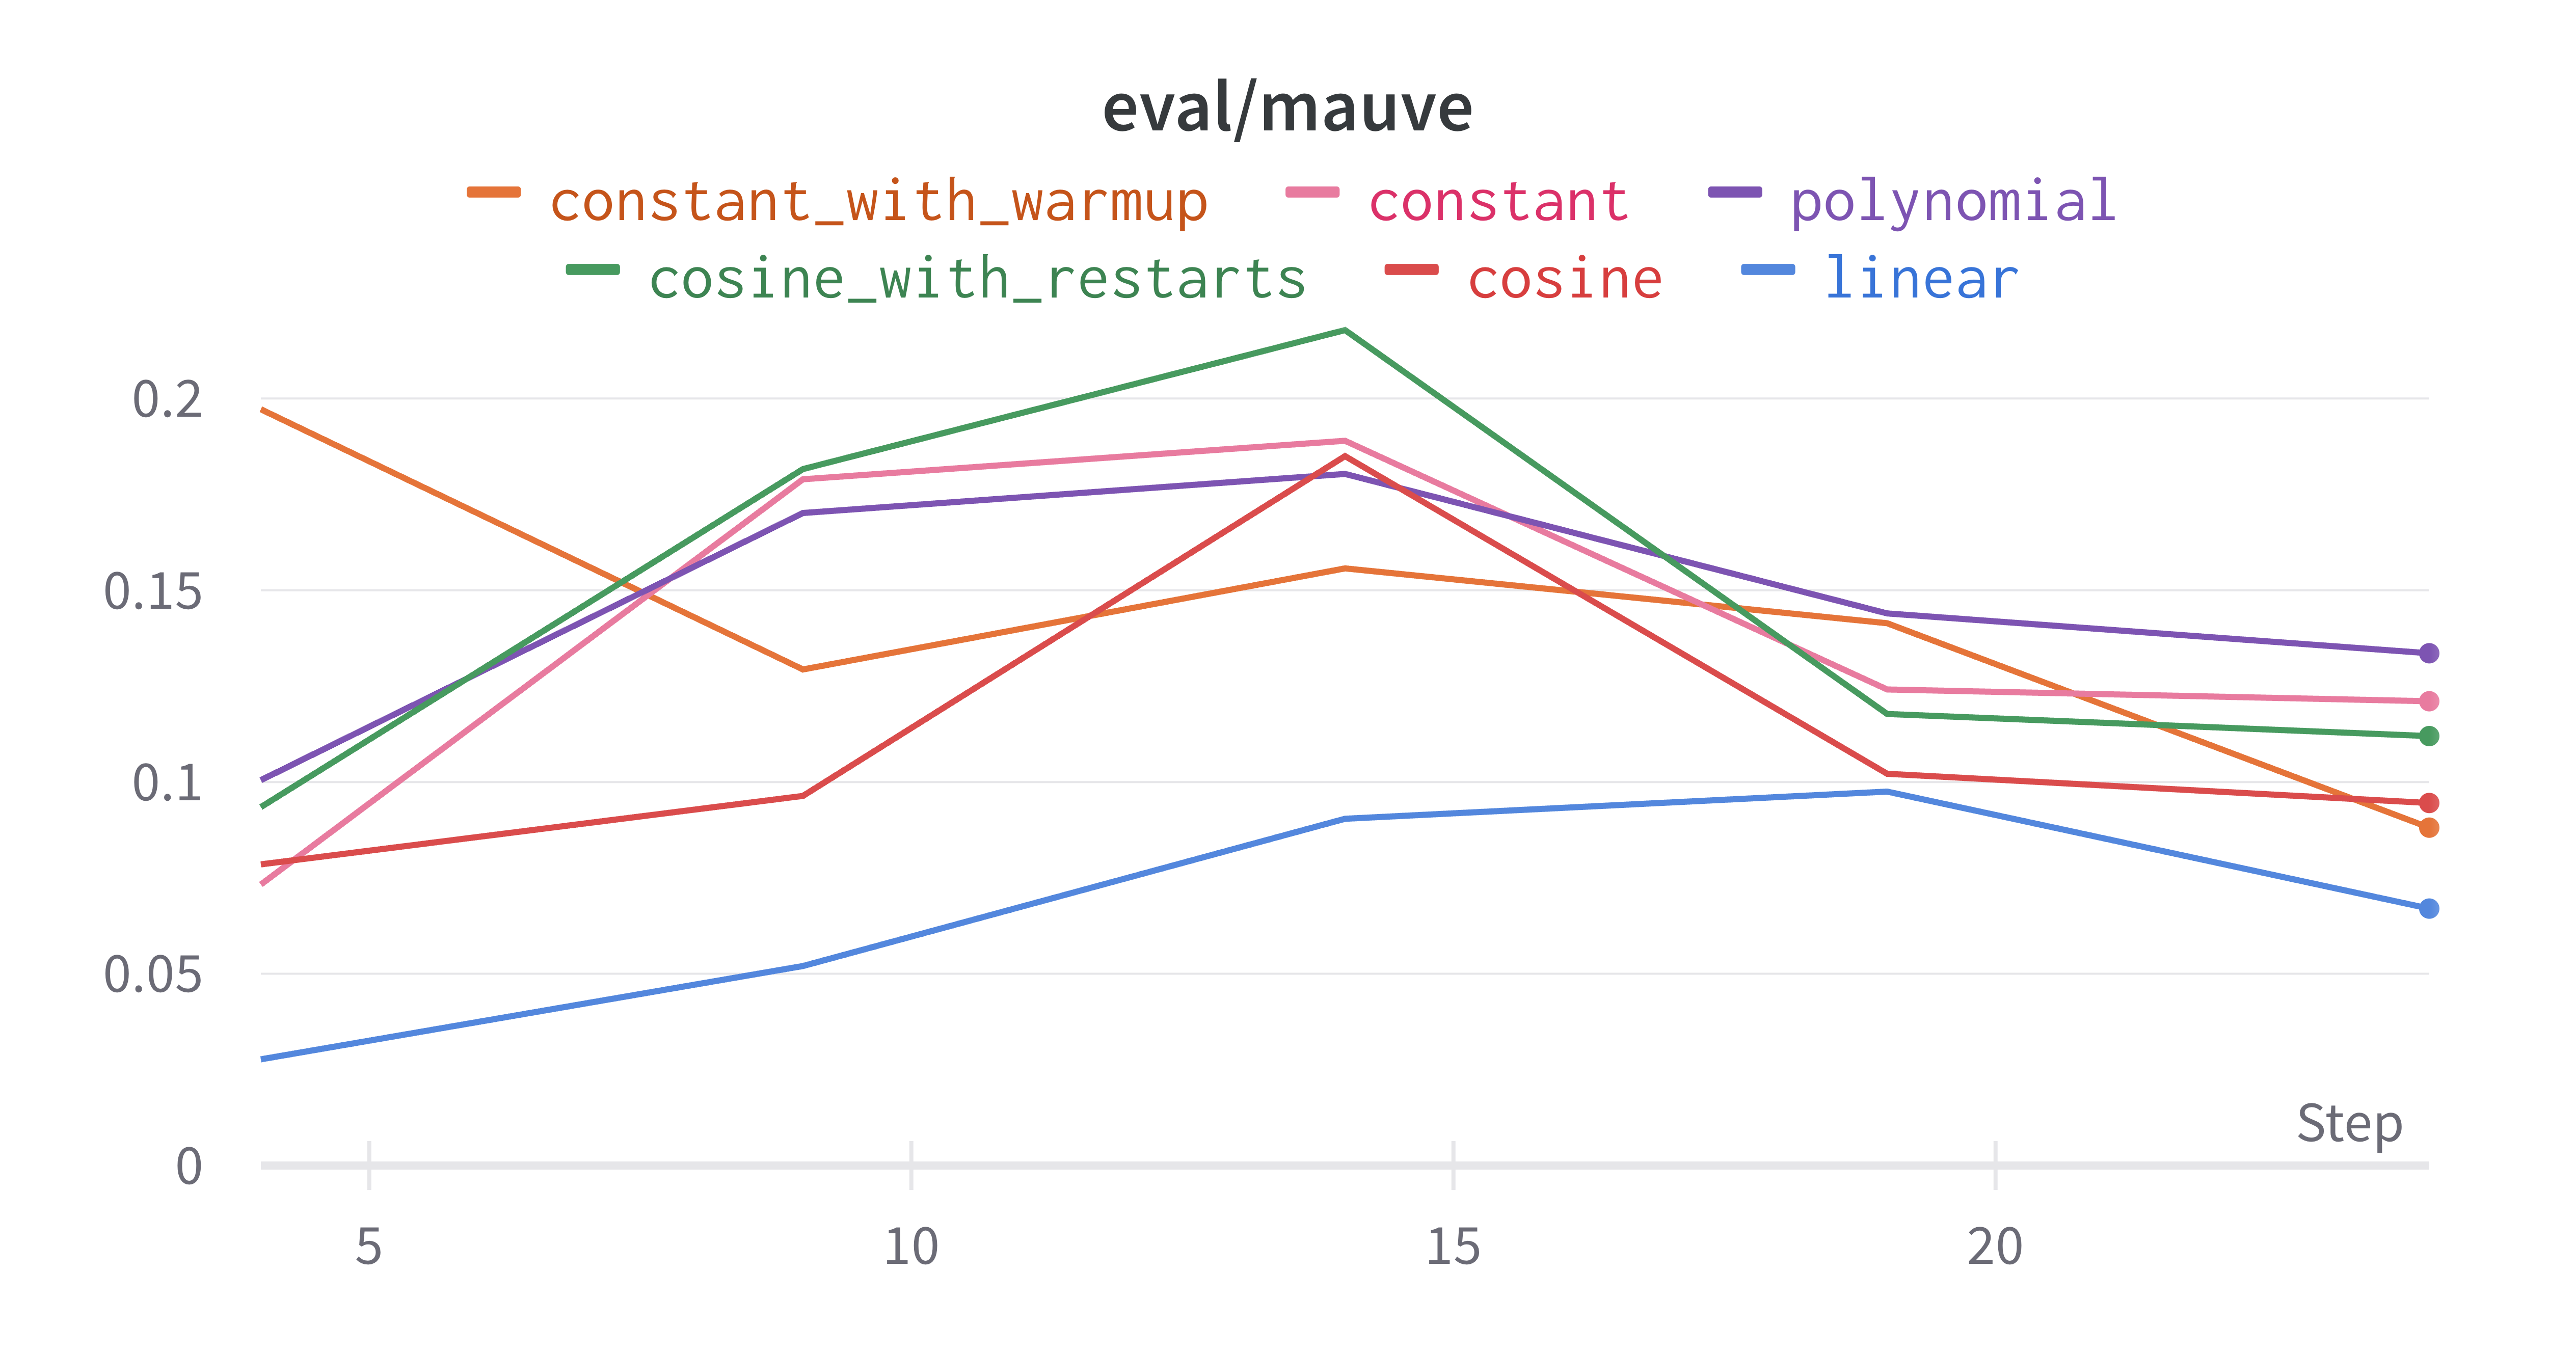
\includegraphics[width=.6\textwidth]{lr-s-mauve}
  \caption{Значение метрики MAUVE на валидационных данных}
  \label{lr-mauve}
\end{figure}

Исходя из всех экспериментов можно сделать вывод, что оптимальные параметры для обучения будут константный планировщик скорости обучения и скорость обучения со значением $9 \times 10{-4}$

\section{ОБУЧЕНИЕ ИТОГОВОЙ МОДЕЛИ}

С подобранными ранее параметрами на была обучена итоговая модель. Общее количество операций, произведенных во время обучения, составило $2 \times 10^{18}$. Количество токенов, которые фигурировали в процессе обучения -- $25 \times 10^{6}$. Процесс обучения виден на рисунках \ref{total-train-loss}, \ref{total-eval-loss}, \ref{total-em}, \ref{total-mauve}. Низкие значения метрик Exact Match и MAUVE можно объяснить сложностью поставленной модели задачи: в диалогах часто ответы формируются исходя из внешних условий, в которых происходился диалог с неигровым персонажем, которые сложно получить из данных игры в формате естественного языка. Метрика Exact Match довольно грубо оценивает результат генерации -- переформулированная фраза в такой оценке даст значение 0. Тем не менее, такую систему получилось обучить на потребительском оборудовании на неплохие результаты. Далее идет пример диалога, который был произведен с моделью.

\texttt{\\Below is the definition of in-game NPC.\\
  The Mad Lord\\
  Alignment: Chaotic Neutral\\
  Description: A mysterious figure who resides in a castle called Caste Maluradek in the middle of a forest. He is a powerful wizard who has the ability to manipulate the elements and create illusions.\\
  Personality traits: He is obsessed with power and will stop at nothing to achieve his goals.\\
  Flaws: He wants to prove that he is the most powerful wizard in the world.
  Motivation: The Mad Lord is a mysterious figure who is driven by his desire for power. He is a master manipulator and will use any means necessary to achieve his goals. He is a powerful wizard who is not afraid to use his magic to get what he wants. He is also a bit of a showman, as he enjoys creating elaborate illusions to impress his guests.\\
  Dialogue history:\\
  Player: START DIALOGUE\\
  NPC: Salutations to the travelers. Welcome to Castle Maluradek. I am your adversary.\\
  Player query: Does the adversary have a name?\\
  Respond to player's query based on defined NPC:\\
  ANSWER: I do not have a name. I am a practitioner of magic. I work in the fields of the great forest.}

Больше примеров можно увидеть в приложении \ref{app:diagogue}.

\begin{figure}[!ht]
  \centering
  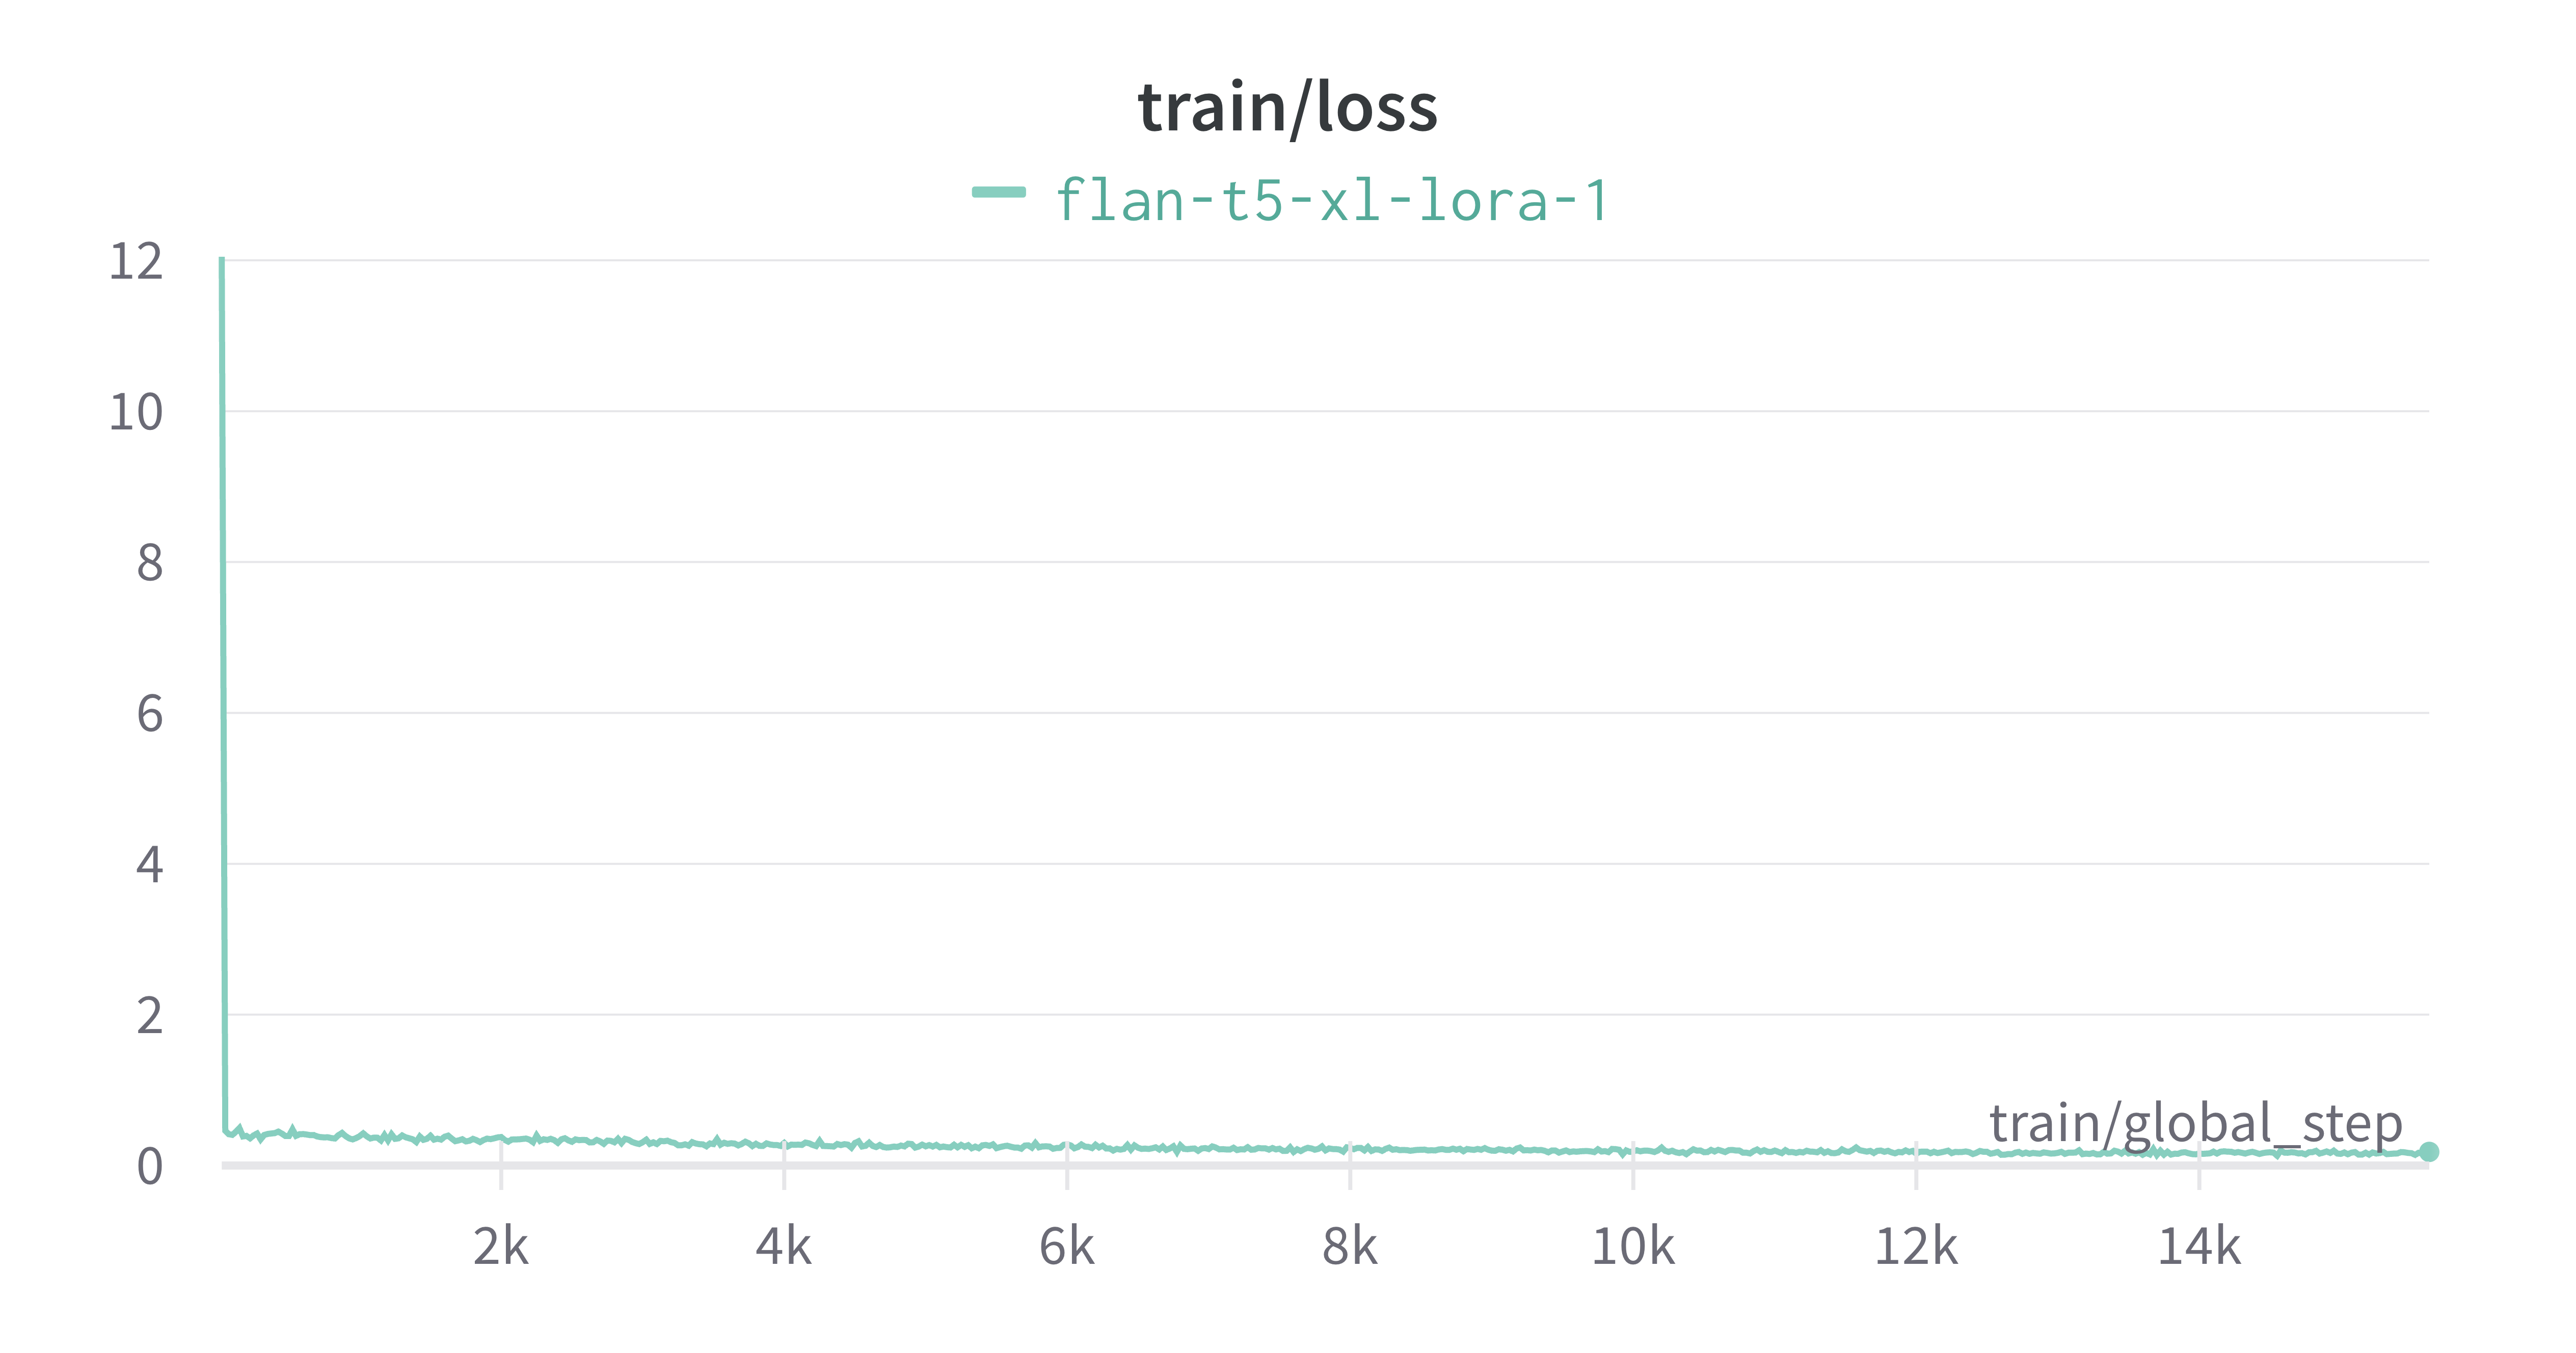
\includegraphics[width=.6\textwidth]{total-train-loss}
  \caption{Значение функции ошибки на тренировочных данных}
  \label{total-train-loss}
\end{figure}

\begin{figure}[!ht]
  \centering
  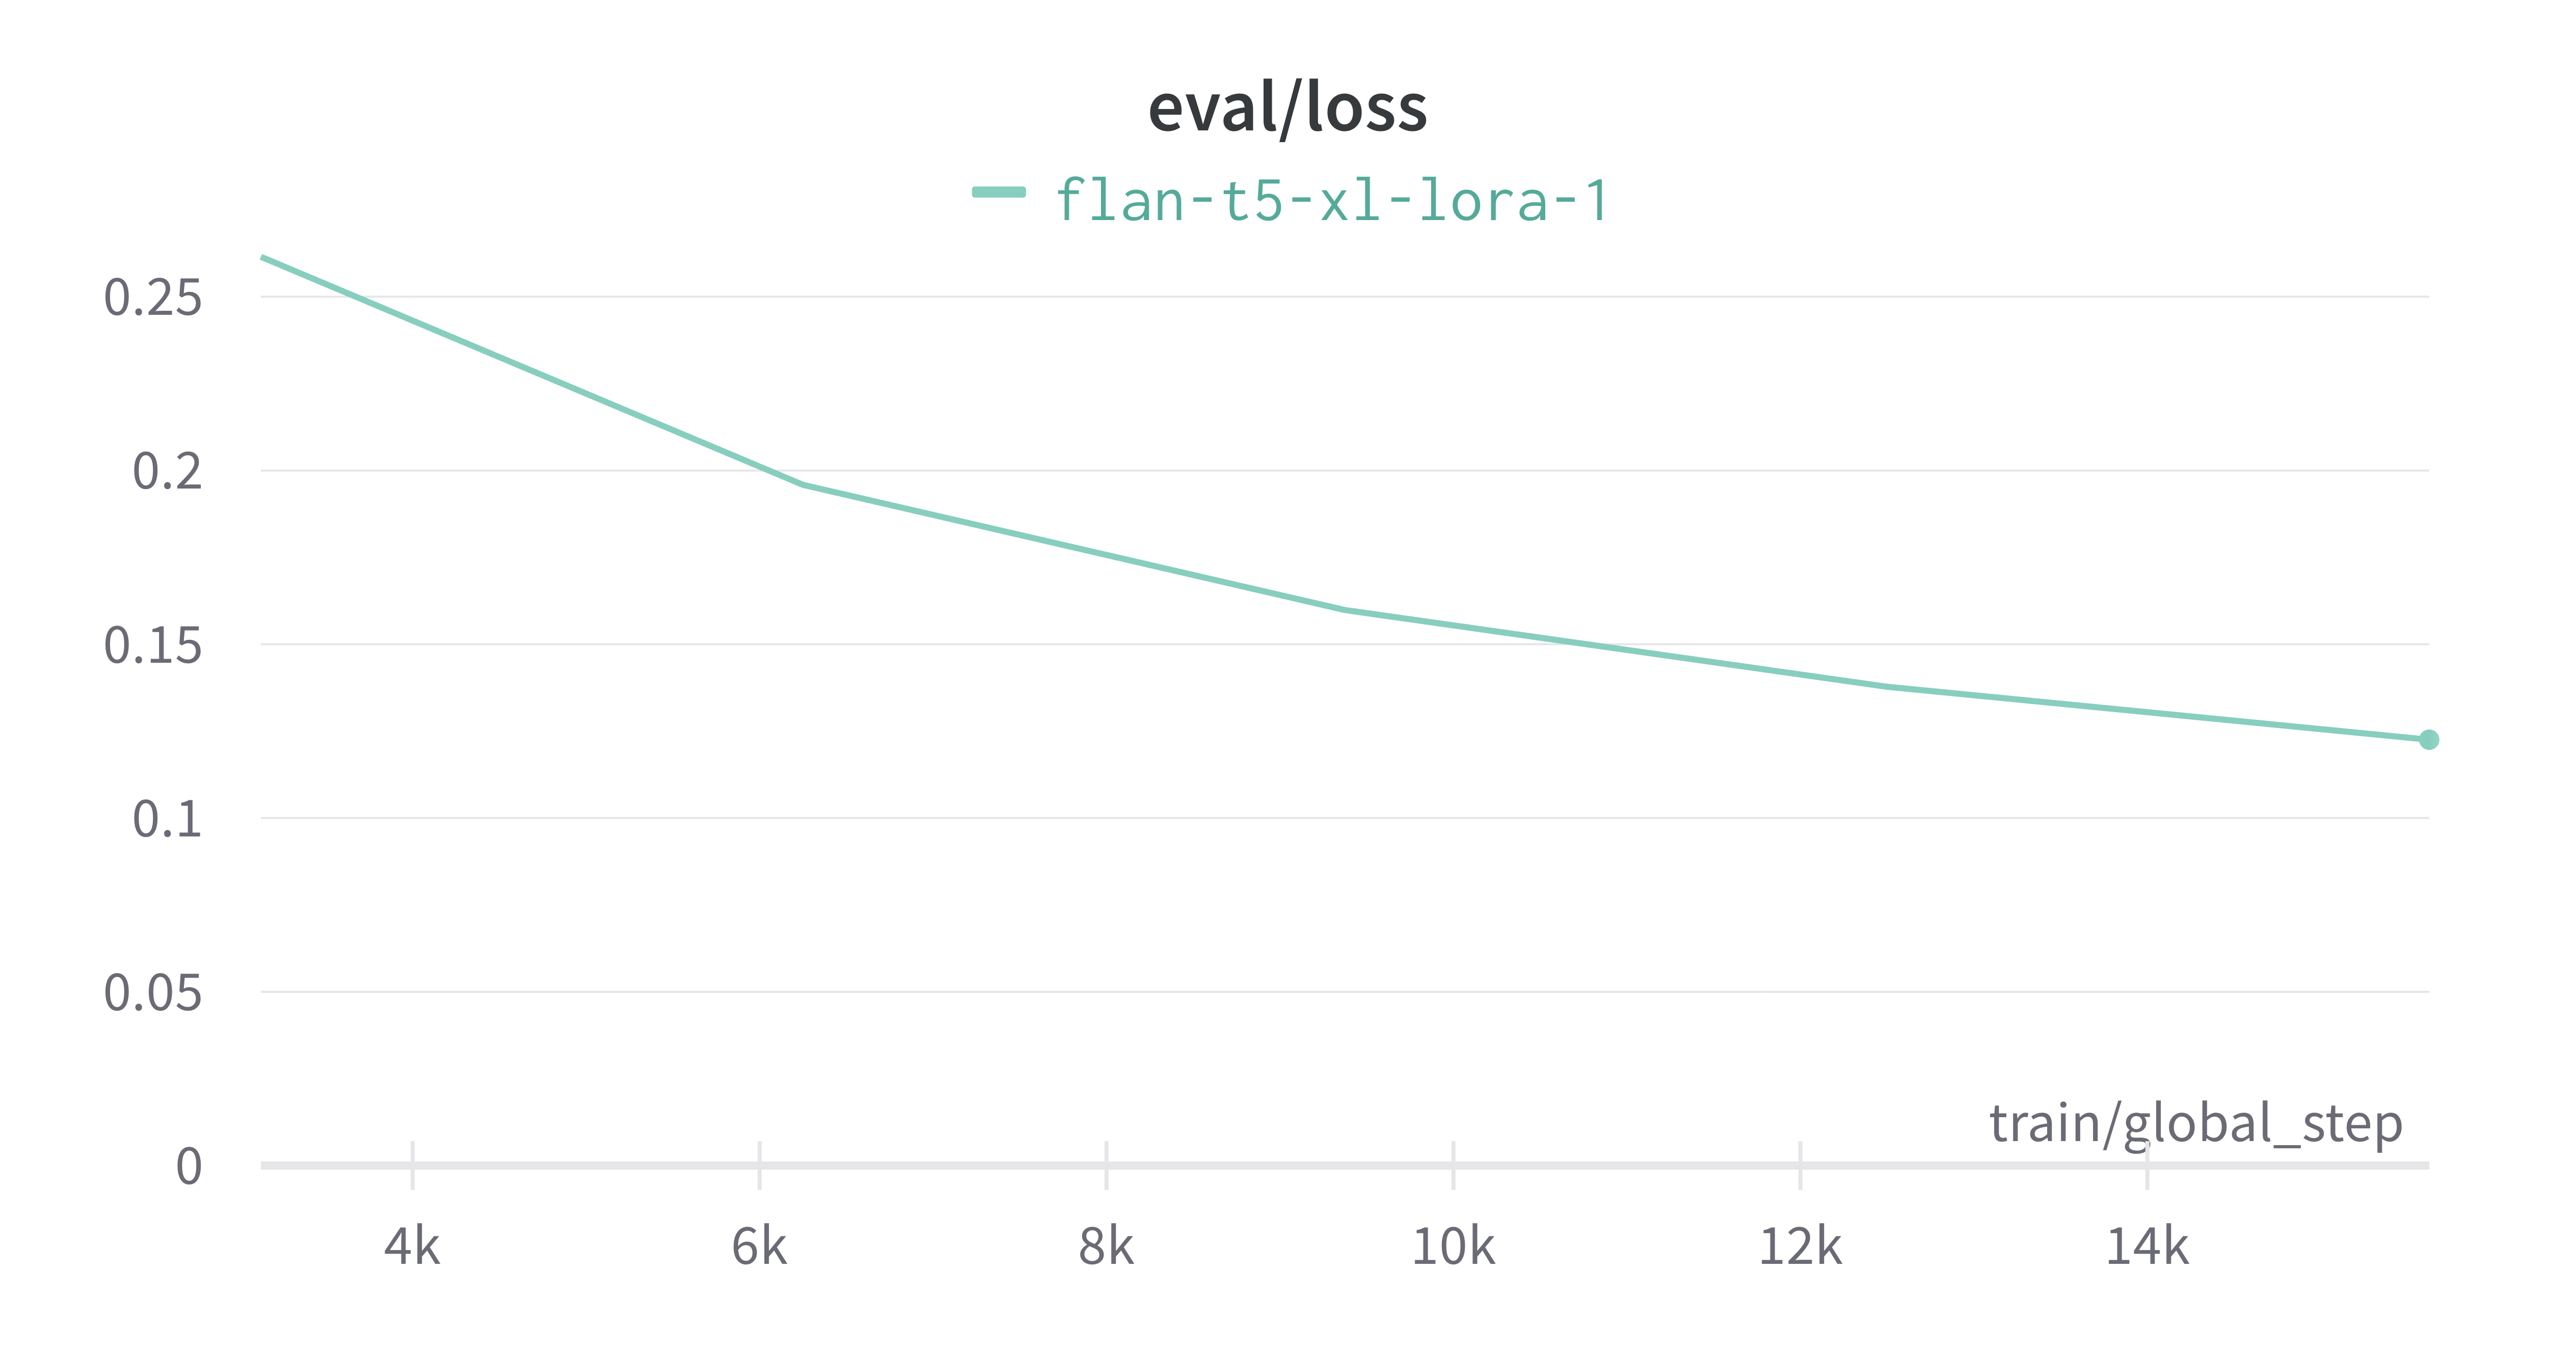
\includegraphics[width=.6\textwidth]{total-eval-loss}
  \caption{Значение функции ошибки на валидационных данных}
  \label{total-eval-loss}
\end{figure}

\begin{figure}[!ht]
  \centering
  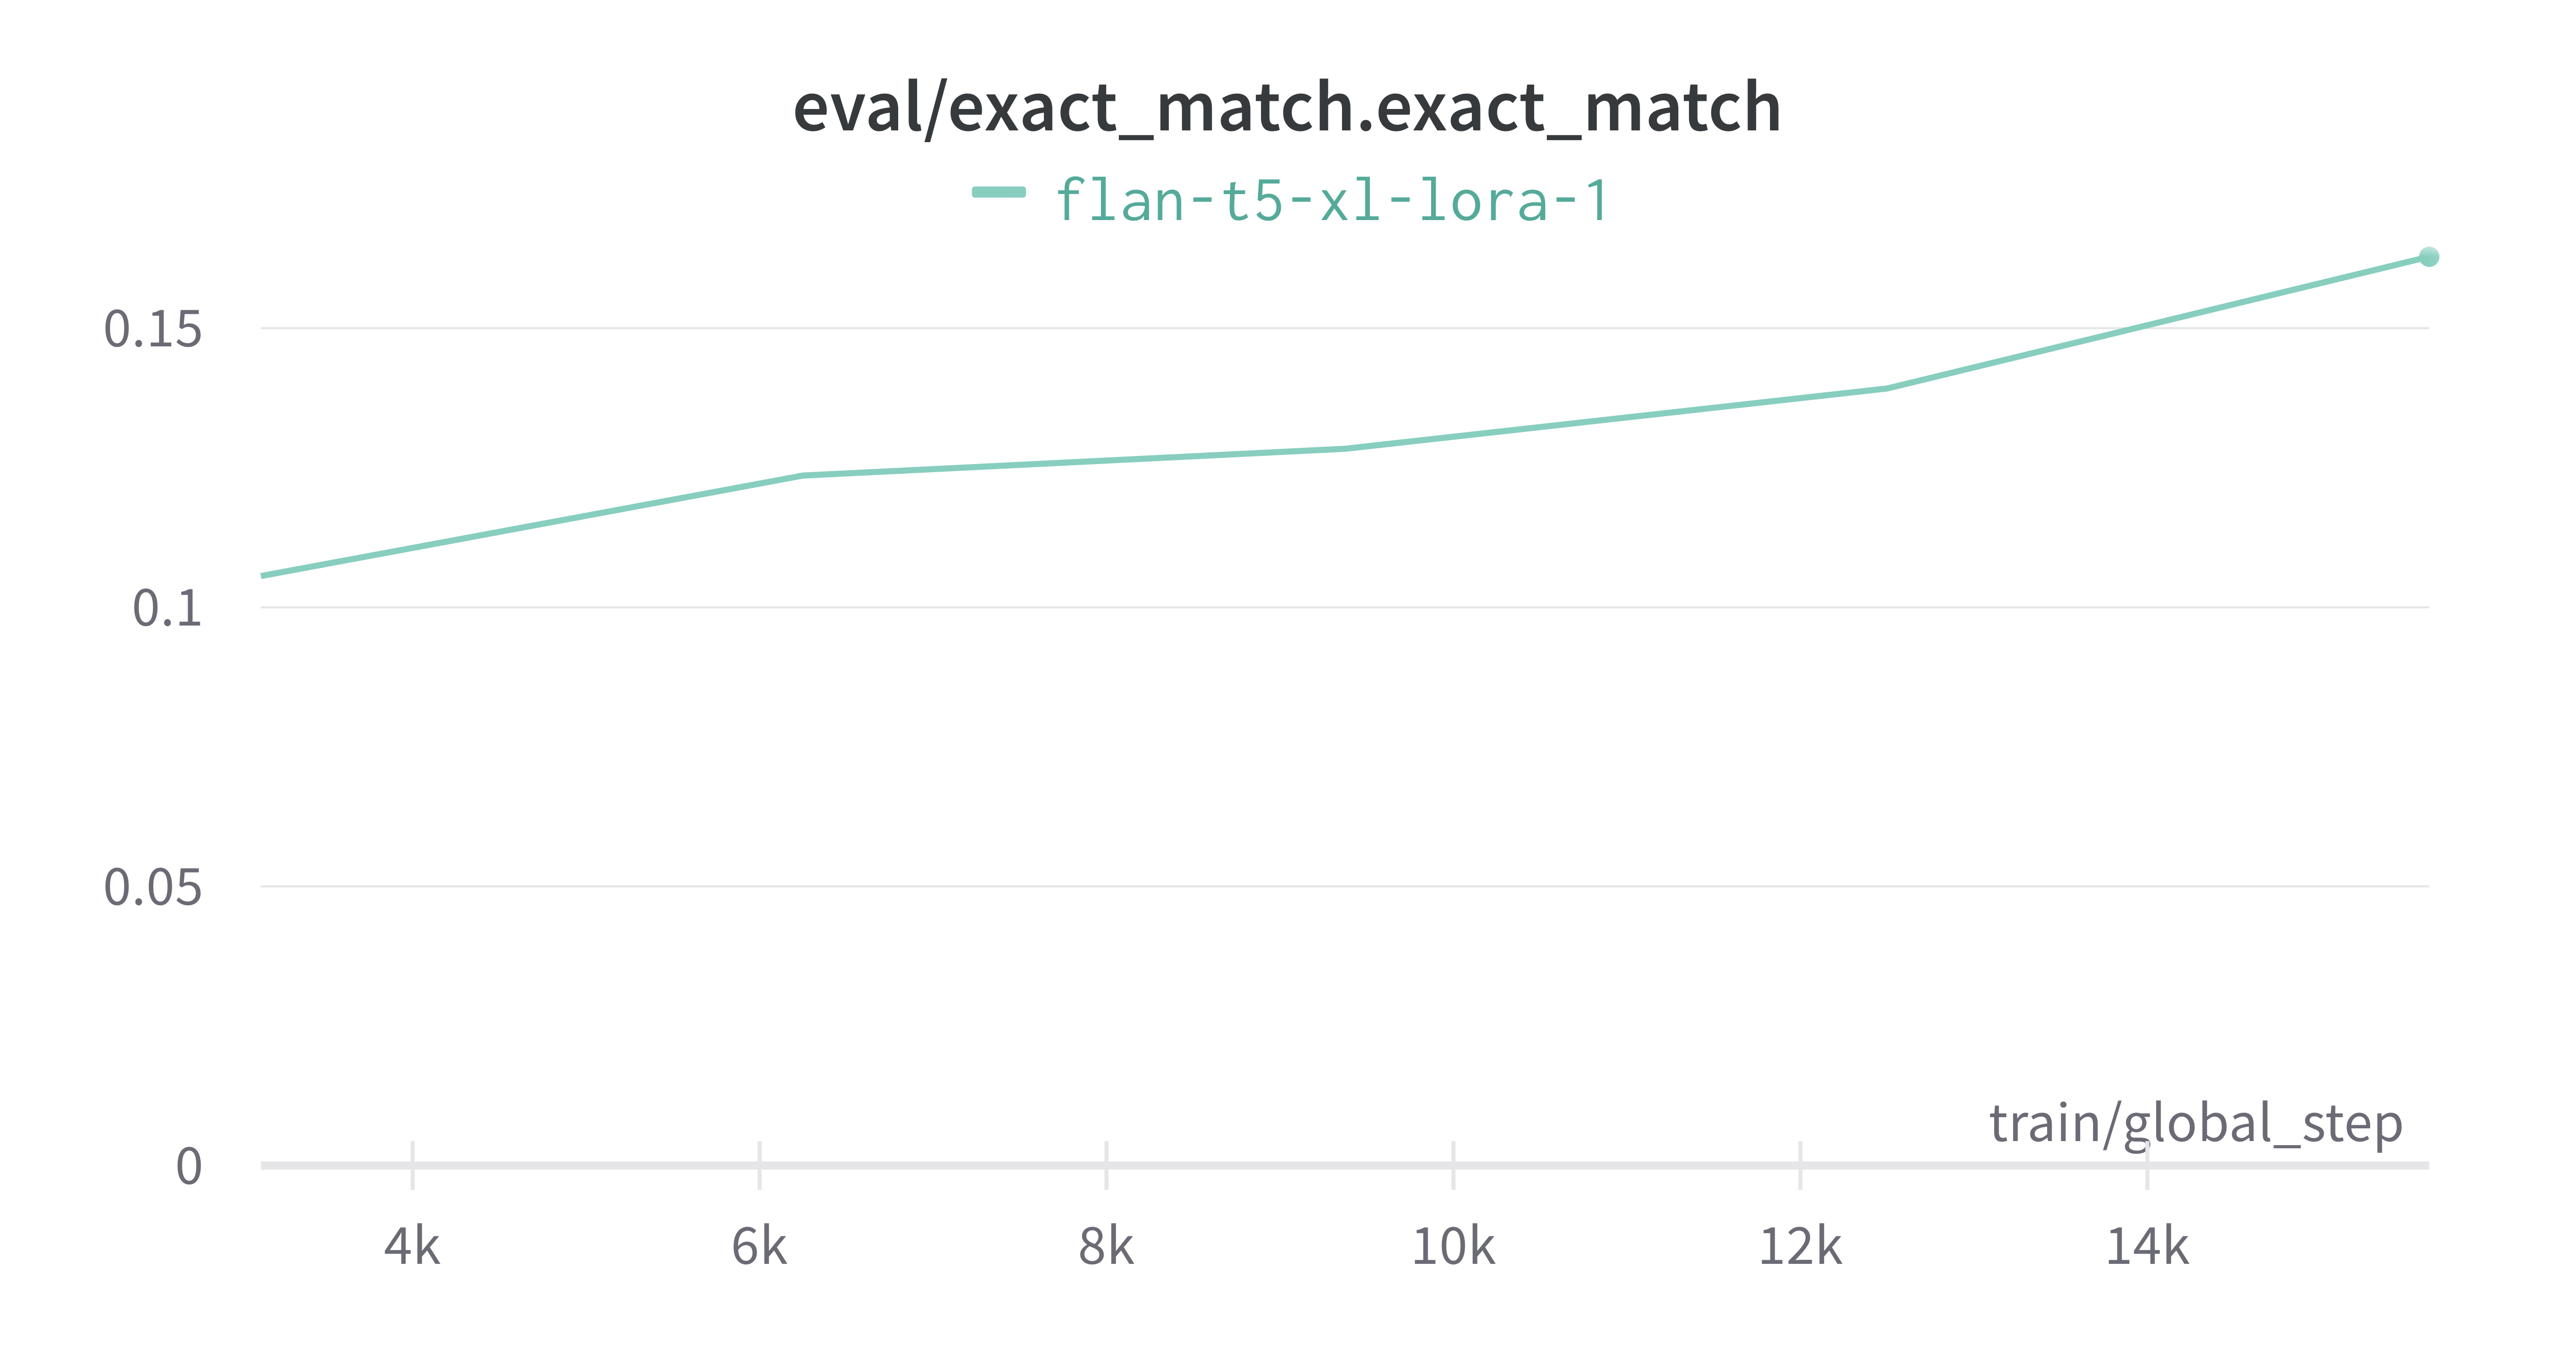
\includegraphics[width=.6\textwidth]{total-em}
  \caption{Значение метрики Exact Match на валидационных данных}
  \label{total-em}
\end{figure}

\begin{figure}[!ht]
  \centering
  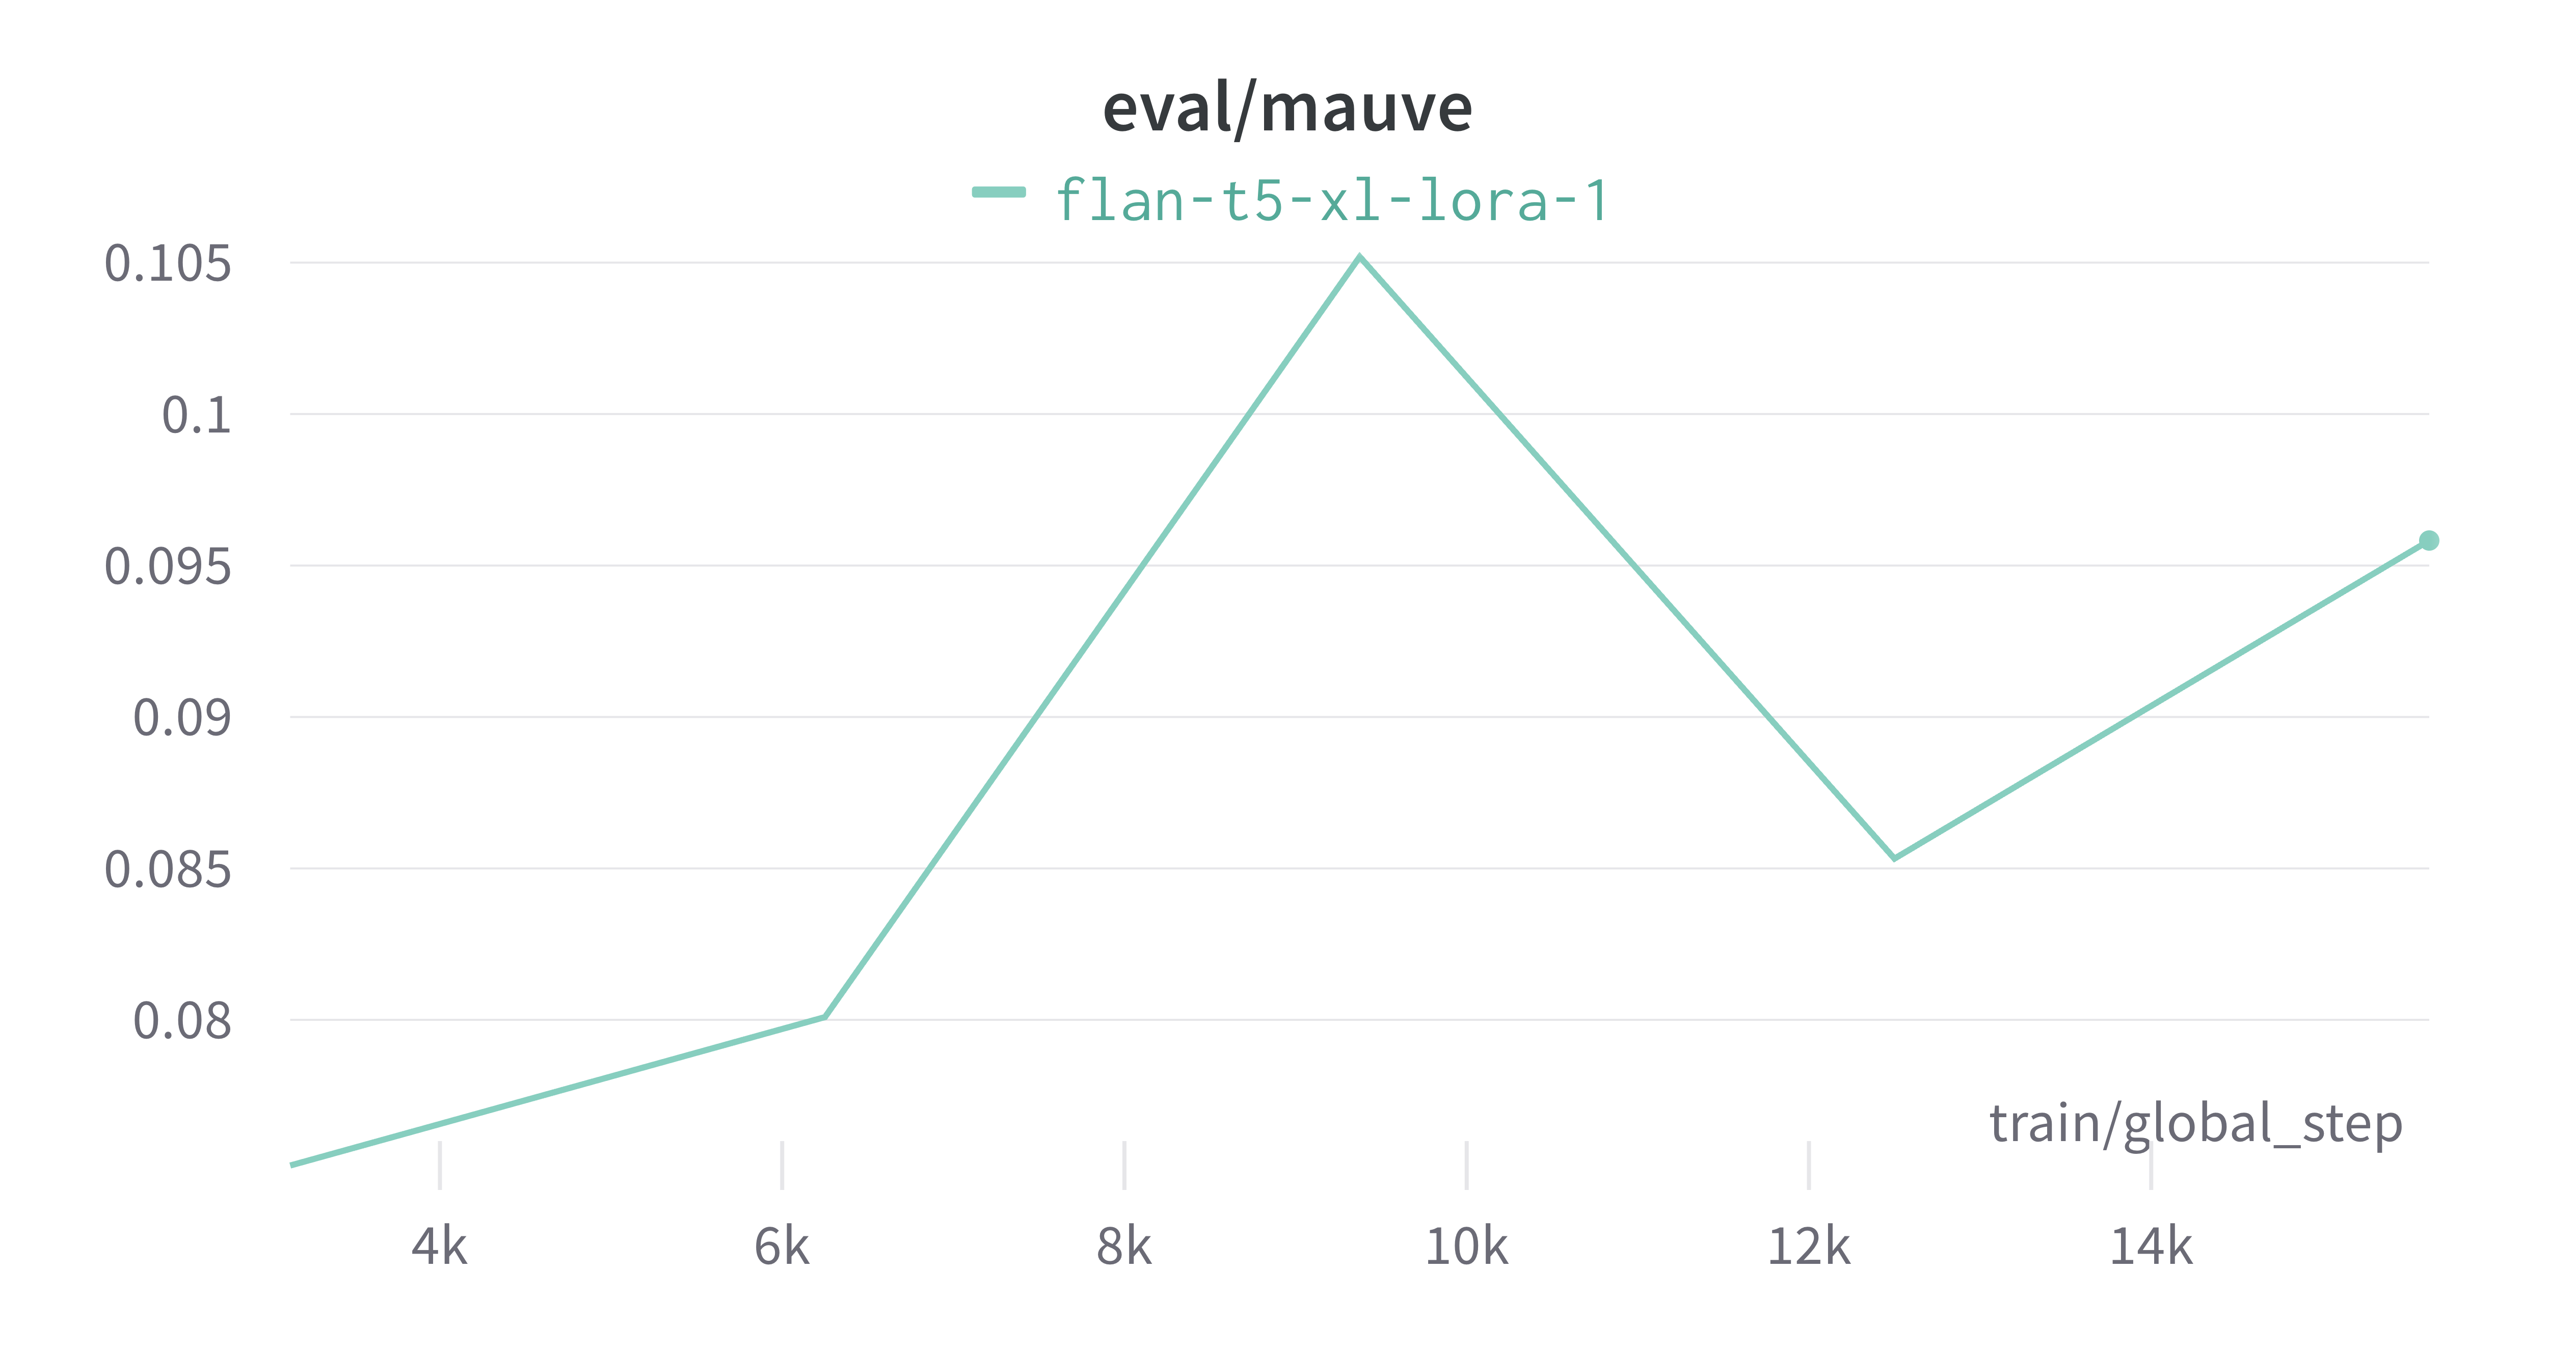
\includegraphics[width=.6\textwidth]{total-mauve}
  \caption{Значение метрики MAUVE на валидационных данных}
  \label{total-mauve}
\end{figure}
